\documentclass[11pt]{article}

% ---------- Packages ----------
\usepackage[a4paper,margin=1in]{geometry}
\usepackage{graphicx}
\usepackage{float}
\usepackage{booktabs}
\usepackage{amsmath}
\usepackage{hyperref}
\usepackage{placeins}
\usepackage{microtype}
\usepackage{setspace}
\usepackage{subcaption}
\usepackage{array}
\usepackage{longtable}
\usepackage{enumitem}

\onehalfspacing

\begin{document}

\begin{titlepage}
    \centering
    \vspace*{2cm}

    {\Huge \textbf{Project Report on}}\\[0.5cm]
    {\LARGE \textbf{Analysis of Online News Popularity Using Machine Learning and Big Data Techniques}}\\[1.5cm]

    {\Large Big Data Analytics}\\[0.3cm]
    {\large under Dr. Hao Cai}\\[2cm]

    \textbf{Submitted by}\\[0.5cm]
    Kuladeep Pappu : 202407268\\
    Tanvish Minache : 202402792\\
    Meet Patel : 202407335\\[2cm]

    \vfill
    {\large \today}
\end{titlepage}


\newpage
\tableofcontents
\newpage

\section*{Abstract}
\addcontentsline{toc}{section}{Abstract}

This project analyzes the Online News Popularity dataset to understand and predict user engagement with online news articles. The study is organized around a set of clearly defined data analytics tasks rather than a purely method-based workflow. These tasks include popularity classification, share prediction, clustering, engagement pattern discovery, formatting analysis, publication timing analysis, and a Spark-based scalability demonstration.

The dataset contains 39,644 articles described by numerical features related to article content, keyword statistics, topic distributions, sentiment, media usage, and publication timing. After data cleaning and exploratory analysis, a structured feature engineering pipeline was applied, including correlation filtering, feature importance ranking, feature selection, and dimensionality reduction. This allowed the analysis to focus on the most informative variables while reducing redundancy in the input space.

Across the predictive tasks, ensemble models such as Gradient Boosting and Random Forest performed better than simpler linear and distance-based methods, indicating that article popularity is influenced by non-linear relationships among features. Exploratory tasks showed that the dataset has limited natural cluster separation, but still revealed useful patterns such as stronger engagement for weekend and technology-related articles. A focused formatting task provided interpretable insights into how links, images, videos, and article length relate to engagement, although these factors alone explain only a limited portion of the variation in shares.

Overall, the project demonstrates how predictive modeling, exploratory analysis, and feature-driven interpretation can be combined within a task-oriented structure to better understand online news popularity. The inclusion of a PySpark workflow further shows how the same analytical pipeline can be extended to scalable distributed environments.

\newpage

\section{Introduction}

The rapid growth of digital media platforms has transformed the way news is produced, consumed, and shared. Online publishers now compete not only for readership, but also for visibility across social media platforms, where article shares strongly influence audience reach and engagement. As a result, understanding the factors that drive online news popularity has become an important problem for content creators, publishers, and digital marketing teams \cite{bishop2006prml,han2011datamining}.

Predicting the popularity of an online article is a challenging task. User engagement is influenced by multiple interacting factors, including article length, language characteristics, topic, sentiment, publication timing, and media elements such as images and videos. These factors do not act independently, and the relationship between article features and popularity is often highly non-linear. This makes online news popularity an appropriate and interesting problem for machine learning and data analytics \cite{bishop2006prml,han2011datamining}.

In this project, the Online News Popularity dataset is used to study how different article characteristics relate to engagement \cite{fernandes2015dataset}. The dataset contains thousands of articles from Mashable, along with numerical features describing content structure, keyword statistics, topic probabilities, sentiment information, publication timing, and the number of social media shares. Because the dataset supports both predictive and exploratory analysis, it provides a strong basis for a broad data analytics study.

\noindent\textbf{As suggested by the professor,} the structure of this report was revised to make the analytical objectives more explicit. Instead of presenting the work mainly as a sequence of machine learning methods, the revised report frames the analysis around clearly defined tasks so that each stage of the project is linked to a specific practical question.

A key aim of this report is to move beyond simply applying algorithms and instead organize the work around meaningful analytical objectives. For that reason, the project is structured around six explicit tasks: predicting whether an article will be popular, predicting the number of shares, discovering natural article groupings, identifying engagement-related feature patterns, analyzing formatting and media usage, and investigating publication timing. This task-oriented structure makes the purpose of each analysis step clearer and aligns the technical methods with real-world questions.

The remainder of the report presents the dataset, defines the analytical tasks, explains the preparation and engineering of the data, describes the methodology used for each task, and discusses the main findings, limitations, and future directions of the study.

\section{Dataset Description}

The dataset used in this project is the \textit{Online News Popularity} dataset from the UCI Machine Learning Repository \cite{fernandes2015dataset}. It contains information about online news articles published by Mashable and is widely used for studying engagement prediction and content analytics.

The working dataset used in this report contains 39,644 rows and 59 columns. Each row represents a single news article, and the target variable is \texttt{shares}, which records the number of times the article was shared on social media. All variables are numeric, which makes the dataset suitable for a wide range of machine learning and data mining techniques.

The features can be grouped into several meaningful categories:

\begin{itemize}[leftmargin=1.5em]
    \item \textbf{Content features:} title length, article length, token statistics, and lexical characteristics.
    \item \textbf{Media and link features:} number of hyperlinks, self-references, images, and videos.
    \item \textbf{Keyword statistics:} measures describing the popularity and distribution of article keywords.
    \item \textbf{Topic features:} latent topic probabilities obtained through LDA-based representations.
    \item \textbf{Sentiment features:} polarity, subjectivity, and positive/negative word ratios.
    \item \textbf{Publication features:} weekday indicators and the weekend flag.
    \item \textbf{Channel indicators:} binary variables describing the article channel, such as technology, entertainment, or business.
\end{itemize}

This dataset is well suited to the project because it supports multiple types of analysis \cite{han2011datamining}. It can be used for classification tasks such as identifying whether an article is popular, for regression tasks such as estimating the number of shares, and for exploratory tasks such as clustering and association rule mining. The diversity of the features also makes it possible to study both predictive performance and practical interpretation.

\section{Task Definition}

To ensure clarity of objectives, the project is organized around six specific data analytics tasks. Each task addresses a meaningful question related to online news popularity and helps connect the technical analysis to real-world interpretation. For each task, the input features, output target, and task type are explicitly stated so that the experimental setup can be reproduced.

\subsection{Task 1: Predicting Whether a News Article Will Be Popular}
\textbf{Real-World Question:} Given an article's content features, can we classify it as popular or unpopular before publication?

\begin{itemize}[leftmargin=1.5em]
    \item \textbf{Type:} Supervised --- Binary Classification
    \item \textbf{Input:} 29 selected features identified through preliminary feature analysis (see Section~\ref{sec:feature_engineering})
    \item \textbf{Output:} Binary label --- Popular (1) if shares $\geq$ median (1400), Unpopular (0) otherwise
\end{itemize}

\subsection{Task 2: Predicting the Number of Shares an Article Will Receive}
\textbf{Real-World Question:} Can we estimate how many shares an article will receive based on its measurable properties?

\begin{itemize}[leftmargin=1.5em]
    \item \textbf{Type:} Supervised --- Regression
    \item \textbf{Input:} Same 29 selected features as Task~1
    \item \textbf{Output:} Continuous value --- $\log(1 + \texttt{shares})$
\end{itemize}

\subsection{Task 3: Discovering Natural Groupings of News Articles}
\textbf{Real-World Question:} Do news articles naturally separate into distinct groups based on their content, sentiment, and structural characteristics?

\begin{itemize}[leftmargin=1.5em]
    \item \textbf{Type:} Unsupervised --- Clustering
    \item \textbf{Input:} 29 selected features (scaled with StandardScaler)
    \item \textbf{Output:} Cluster labels assigned by K-Means and DBSCAN
\end{itemize}

\subsection{Task 4: Identifying Content Patterns Associated with High Engagement}
\textbf{Real-World Question:} What combinations of article properties (weekend, channel, topic) tend to co-occur in highly shared articles?

\begin{itemize}[leftmargin=1.5em]
    \item \textbf{Type:} Unsupervised --- Association Rule Mining
    \item \textbf{Input:} Binary indicator features (weekday flags, channel flags, binarized popularity target)
    \item \textbf{Output:} Association rules with support, confidence, and lift scores
\end{itemize}

\subsection{Task 5: Optimizing Article Formatting and Media Usage for Maximum Reach}
\textbf{Real-World Question:} What is the optimal combination of text length, links, and media (images/videos) to drive shares?

\begin{itemize}[leftmargin=1.5em]
    \item \textbf{Type:} Supervised --- Regression (with focus on feature coefficients)
    \item \textbf{Input:} 6 structural formatting features only: \texttt{n\_tokens\_title}, \texttt{n\_tokens\_content}, \texttt{num\_imgs}, \texttt{num\_videos}, \texttt{num\_hrefs}, \texttt{num\_self\_hrefs}
    \item \textbf{Output:} Continuous value --- $\log(1 + \texttt{shares})$
\end{itemize}

\subsection{Task 6: Recommending the Optimal Publication Window (Weekday vs.\ Weekend)}
\textbf{Real-World Question:} Given the emotional tone and topic of a drafted article, is it better suited for a weekday or weekend release?

\begin{itemize}[leftmargin=1.5em]
    \item \textbf{Type:} Supervised --- Binary Classification
    \item \textbf{Input:} 26 features: 16 NLP/sentiment features, 5 channel indicators, and 5 LDA topic features (Latent Dirichlet Allocation topic closeness scores)
    \item \textbf{Output:} Binary label --- Weekday (0) or Weekend (1)
\end{itemize}

\noindent\textit{Note: The dataset does not contain hour-level publication timestamps; only weekday indicator columns are available. Therefore, this task uses weekday vs.\ weekend as the temporal dimension rather than a 24-hour analysis.}


\section{Data Preparation}

\subsection{Data Cleaning}

The dataset was systematically inspected for quality issues before any modeling. Each cleaning step was performed explicitly and its result documented to ensure full transparency.

\begin{table}[H]
\centering
\caption{Data cleaning summary}
\begin{tabular}{lll}
\toprule
\textbf{Check} & \textbf{Finding} & \textbf{Action Taken} \\
\midrule
Missing values & 0 across all 61 columns & No imputation needed \\
Duplicate rows & 0 duplicates found & No removal needed \\
Non-numeric columns & \texttt{url} (string) & Dropped (non-predictive) \\
Non-predictive columns & \texttt{url}, \texttt{timedelta} & Dropped (2 columns removed) \\
Data types & All 59 remaining columns numeric & No encoding needed \\
Binary indicators & 13 columns (weekday, channel flags) & Used as-is \\
Outliers (\texttt{shares}) & IQR method: 10,072 outliers (25.4\%) & \textbf{Not removed} (see below) \\
\bottomrule
\end{tabular}
\end{table}

\noindent The target variable \texttt{shares} showed a strongly right-skewed distribution (min: 1, max: 843,300, median: 1,400). Using the IQR method, 25.4\% of articles were flagged as outliers. These outliers were \textbf{not removed} because they reflect the natural behavior of online engagement, where a small number of articles can become highly viral. Instead, the skewness was handled during regression tasks using the transformation $\log(1 + \texttt{shares})$, which stabilizes the variance while preserving the data structure.

After cleaning, the working dataset contained \textbf{39,644 rows} and \textbf{59 numeric columns} (58 features + 1 target).

\subsection{Preprocessing: Before vs.\ After}
\label{sec:preprocessing_definition}

To study the impact of preprocessing on model performance, all supervised tasks (Tasks~1, 2, 5, and 6) were evaluated under two conditions:

\begin{itemize}[leftmargin=1.5em]
    \item \textbf{Before Preprocessing (Raw):} Features were imputed using median values (via \texttt{SimpleImputer}) but \textit{not scaled}. This tests how models perform on the original feature magnitudes.
    \item \textbf{After Preprocessing (Processed):} Features were imputed with medians and then standardized using \texttt{StandardScaler} (zero mean, unit variance). This benefits scale-sensitive models such as Logistic Regression, KNN, and SVM.
\end{itemize}

\noindent Both conditions used the same train/test split (80/20, stratified for classification, random seed = 42) to ensure a fair comparison.

\subsection{Exploratory Data Analysis}
Exploratory Data Analysis (EDA) was conducted to understand the overall behavior of the dataset before feature engineering and model training, following standard data mining practice \cite{han2011datamining,bishop2006prml}.

The distribution of \texttt{shares} was found to be heavily right-skewed, with most articles receiving relatively modest engagement and a much smaller number receiving extremely high shares. This observation justified the use of log transformation in the regression setting.

\begin{figure}[H]
    \centering
    
\includegraphics[width=0.75\textwidth]{figures/fig1_hist_shares.png}
    \caption{Histogram of article shares showing the strong right-skewed distribution of the target variable.}
    \label{fig:hist_shares}
\end{figure}

\begin{figure}[H]
    \centering
    
\includegraphics[width=0.55\textwidth]{figures/fig2_boxplot_shares.png}
    \caption{Boxplot of article shares highlighting the presence of many extreme outliers.}
    \label{fig:boxplot_shares}
\end{figure}

Correlation analysis showed moderate to strong relationships among some groups of features, especially within keyword-related variables and certain self-reference statistics. This suggested the presence of redundancy in the original feature space and motivated the need for feature selection.

\begin{figure}[H]
    \centering
    
\includegraphics[width=0.82\textwidth]{figures/fig3_correlation_heatmap.png}
    \caption{Correlation heatmap of selected numerical features before feature selection.}
    \label{fig:corr_heatmap_before}
\end{figure}

Additional descriptive analysis indicated that articles published on weekends tend to receive somewhat higher engagement on average than those published on weekdays. This observation later informed the association rule and publication timing tasks.

\begin{figure}[H]
    \centering
    
\includegraphics[width=0.72\textwidth]{figures/fig4_scatter_plot.png}
    \caption{Scatter plot showing the relationship between article length and number of shares.}
    \label{fig:scatter_tokens_shares}
\end{figure}

\begin{figure}[H]
    \centering
    
\includegraphics[width=0.7\textwidth]{figures/fig5_bar_chart.png}
    \caption{Average shares by publication day, showing slightly stronger engagement on weekends.}
    \label{fig:weekday_bar}
\end{figure}

\begin{figure}[H]
    \centering
    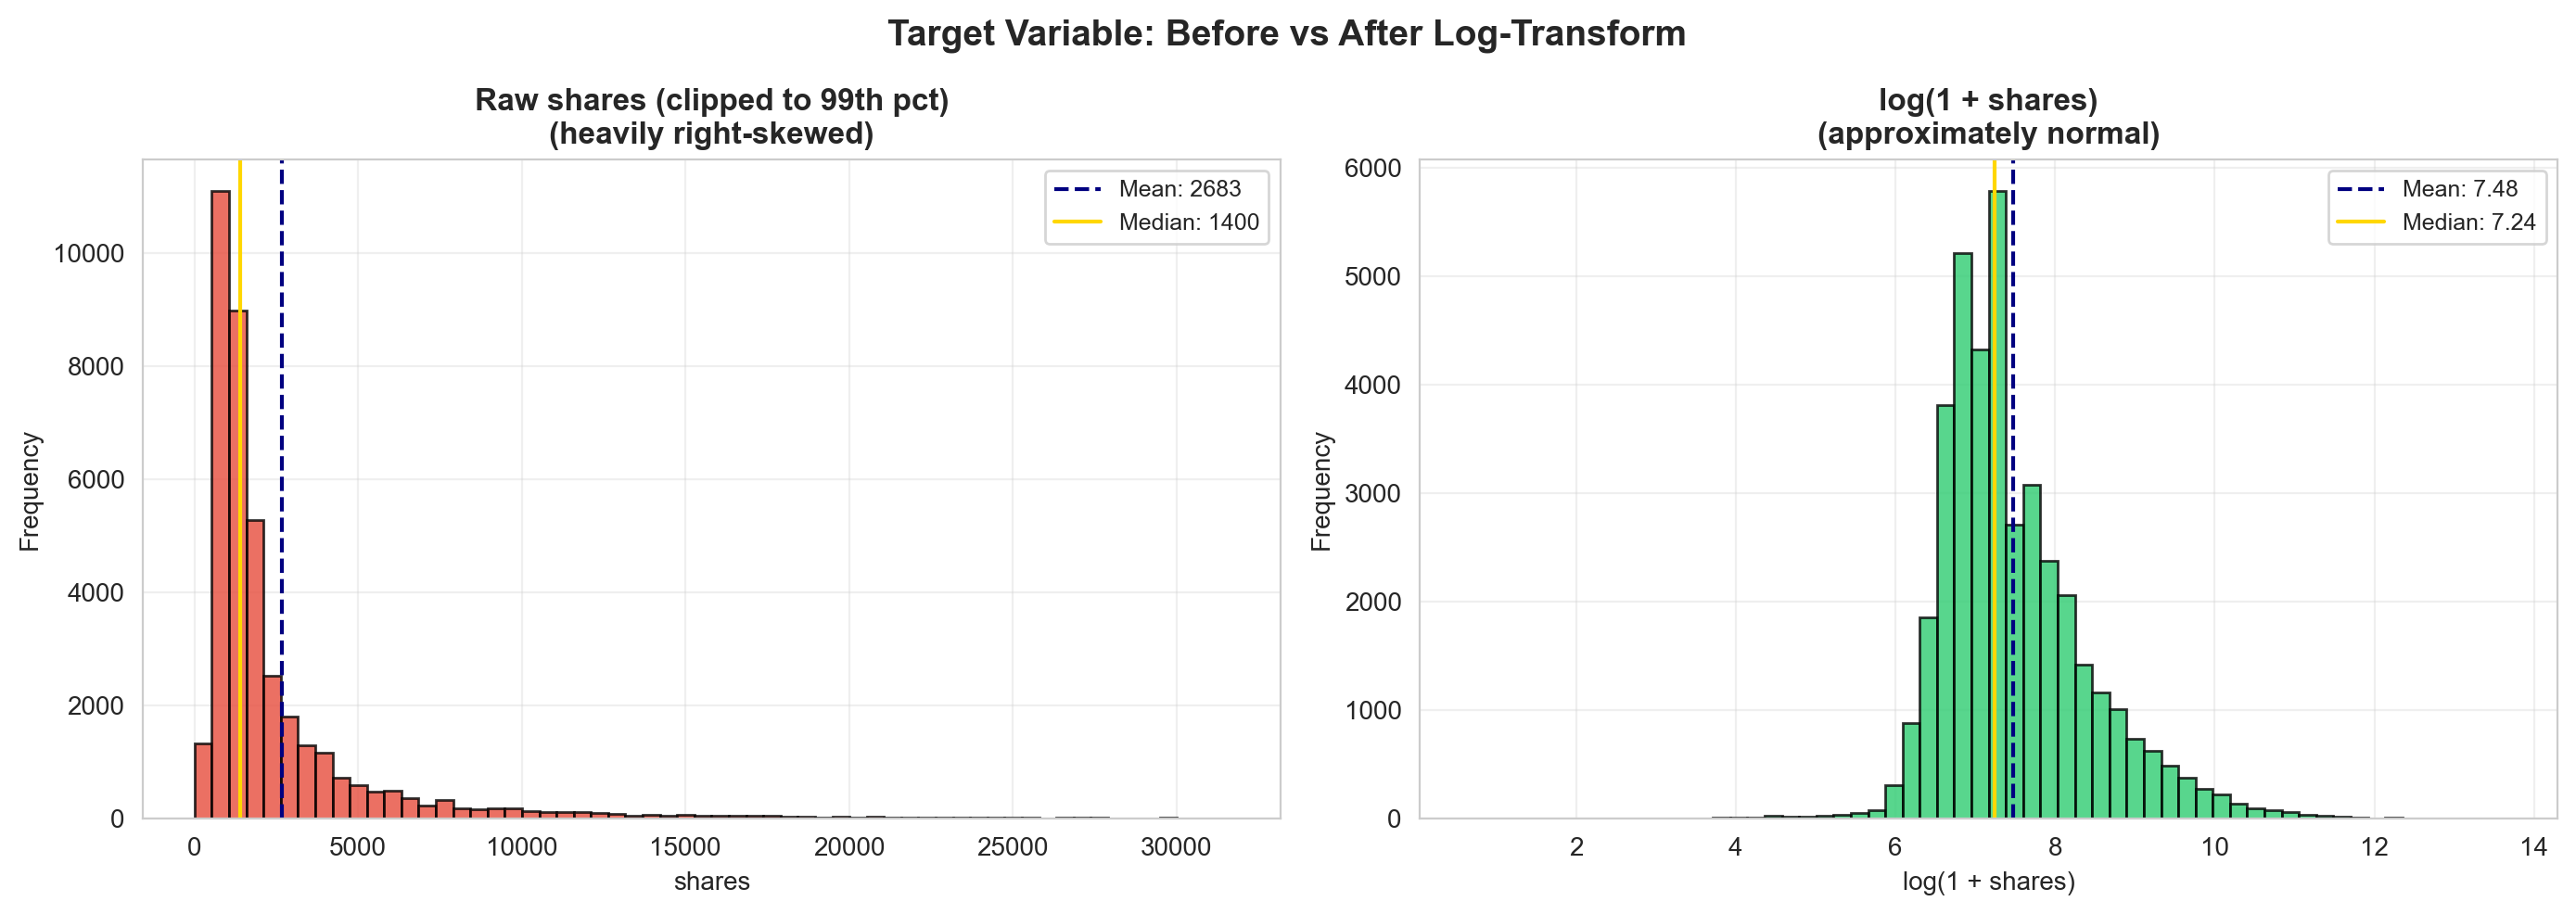
\includegraphics[width=0.9\textwidth]{figures/exp_fig1_shares_vs_log_shares.png}
    \caption{Comparison of the raw \texttt{shares} distribution and the log-transformed target used in regression tasks.}
    \label{fig:shares_vs_logshares}
\end{figure}

Overall, the EDA stage helped identify three key properties of the dataset: skewness in the target variable, redundancy among some predictors, and mild temporal variation in engagement. These findings guided the feature engineering and modeling choices used in later sections.


\section{Feature Engineering}
\label{sec:feature_engineering}

\subsection{Preliminary Feature Analysis and Selection}

\noindent\fbox{\parbox{\dimexpr\textwidth-2\fboxsep-2\fboxrule}{%
\textbf{Key Pipeline (as required by the professor):} The feature engineering followed a strict ordering:
\textbf{(1)}~Correlation-based filtering to remove redundant features,
\textbf{(2)}~Random Forest importance ranking to identify the most predictive features,
\textbf{(3)}~Data-driven selection of the top features using a cumulative importance threshold of 90\%,
and \textbf{(4)}~PCA and t-SNE applied \textit{only} on the selected feature subset.
This ensures that dimensionality reduction is performed after the most important features have been identified, not before.
}}

\bigskip

\subsubsection*{Step 1: Correlation-Based Filtering}

First, pairwise Pearson correlations were computed across all 58 numeric features. Feature pairs with correlation above 0.75 were identified, and the less important feature in each pair was removed. This step eliminated 9 redundant features, reducing the feature space from 58 to 49 columns. The removed features were: \texttt{n\_non\_stop\_words}, \texttt{n\_non\_stop\_unique\_tokens}, \texttt{kw\_avg\_min}, \texttt{kw\_max\_max}, \texttt{kw\_avg\_avg}, \texttt{self\_reference\_avg\_sharess}, \texttt{LDA\_00}, \texttt{LDA\_02}, and \texttt{rate\_negative\_words}.

\begin{figure}[H]
    \centering
    
\includegraphics[width=0.8\textwidth]{figures/fig_correlation_after_removal.png}
    \caption{Correlation structure after removing highly correlated features, showing a more compact and less redundant feature set.}
    \label{fig:corr_after_removal}
\end{figure}

\subsubsection*{Step 2: Random Forest Importance Ranking}

A Random Forest model (200 trees, max depth 15, random seed 42) was trained on all 49 remaining features to compute Gini importance scores \cite{breiman2001rf,biau2016rf}. The features were ranked from most to least important based on these scores.

\subsubsection*{Step 3: Data-Driven Feature Selection}

\textbf{The number of features was not hardcoded}; instead, it was determined by a cumulative importance threshold of 90\%. Starting from the most important feature, features were added until their cumulative importance reached at least 90\% of the total. This resulted in \textbf{29 selected features} covering 90.7\% of the total importance. The selection is bounded between 10 and 35 features as a safeguard.

The 29 selected features, ranked by importance, are:

\begin{longtable}{rll}
\toprule
\textbf{Rank} & \textbf{Feature Name} & \textbf{Importance} \\
\midrule
\endhead
1  & \texttt{kw\_max\_avg} & 0.1077 \\
2  & \texttt{n\_tokens\_content} & 0.0755 \\
3  & \texttt{average\_token\_length} & 0.0640 \\
4  & \texttt{kw\_avg\_max} & 0.0579 \\
5  & \texttt{LDA\_03} & 0.0496 \\
6  & \texttt{kw\_max\_min} & 0.0412 \\
7  & \texttt{self\_reference\_max\_shares} & 0.0389 \\
8  & \texttt{LDA\_04} & 0.0382 \\
9  & \texttt{self\_reference\_min\_shares} & 0.0365 \\
10 & \texttt{LDA\_01} & 0.0315 \\
11 & \texttt{avg\_negative\_polarity} & 0.0314 \\
12 & \texttt{n\_unique\_tokens} & 0.0278 \\
13 & \texttt{global\_subjectivity} & 0.0231 \\
14 & \texttt{global\_sentiment\_polarity} & 0.0226 \\
15 & \texttt{title\_subjectivity} & 0.0223 \\
16 & \texttt{avg\_positive\_polarity} & 0.0219 \\
17 & \texttt{num\_imgs} & 0.0218 \\
18 & \texttt{num\_hrefs} & 0.0217 \\
19 & \texttt{title\_sentiment\_polarity} & 0.0209 \\
20 & \texttt{kw\_min\_avg} & 0.0174 \\
21 & \texttt{num\_self\_hrefs} & 0.0172 \\
22 & \texttt{data\_channel\_is\_bus} & 0.0171 \\
23 & \texttt{global\_rate\_positive\_words} & 0.0169 \\
24 & \texttt{max\_negative\_polarity} & 0.0164 \\
25 & \texttt{n\_tokens\_title} & 0.0160 \\
26 & \texttt{global\_rate\_negative\_words} & 0.0148 \\
27 & \texttt{min\_negative\_polarity} & 0.0132 \\
28 & \texttt{rate\_positive\_words} & 0.0120 \\
29 & \texttt{num\_videos} & 0.0110 \\
\bottomrule
\end{longtable}

\begin{figure}[H]
    \centering
    
\includegraphics[width=0.62\textwidth]{figures/fig_feature_selection.png}
    \caption{Selected features ranked by Random Forest Gini importance. Green bars indicate selected features.}
    \label{fig:feature_selection}
\end{figure}

\begin{figure}[H]
    \centering
    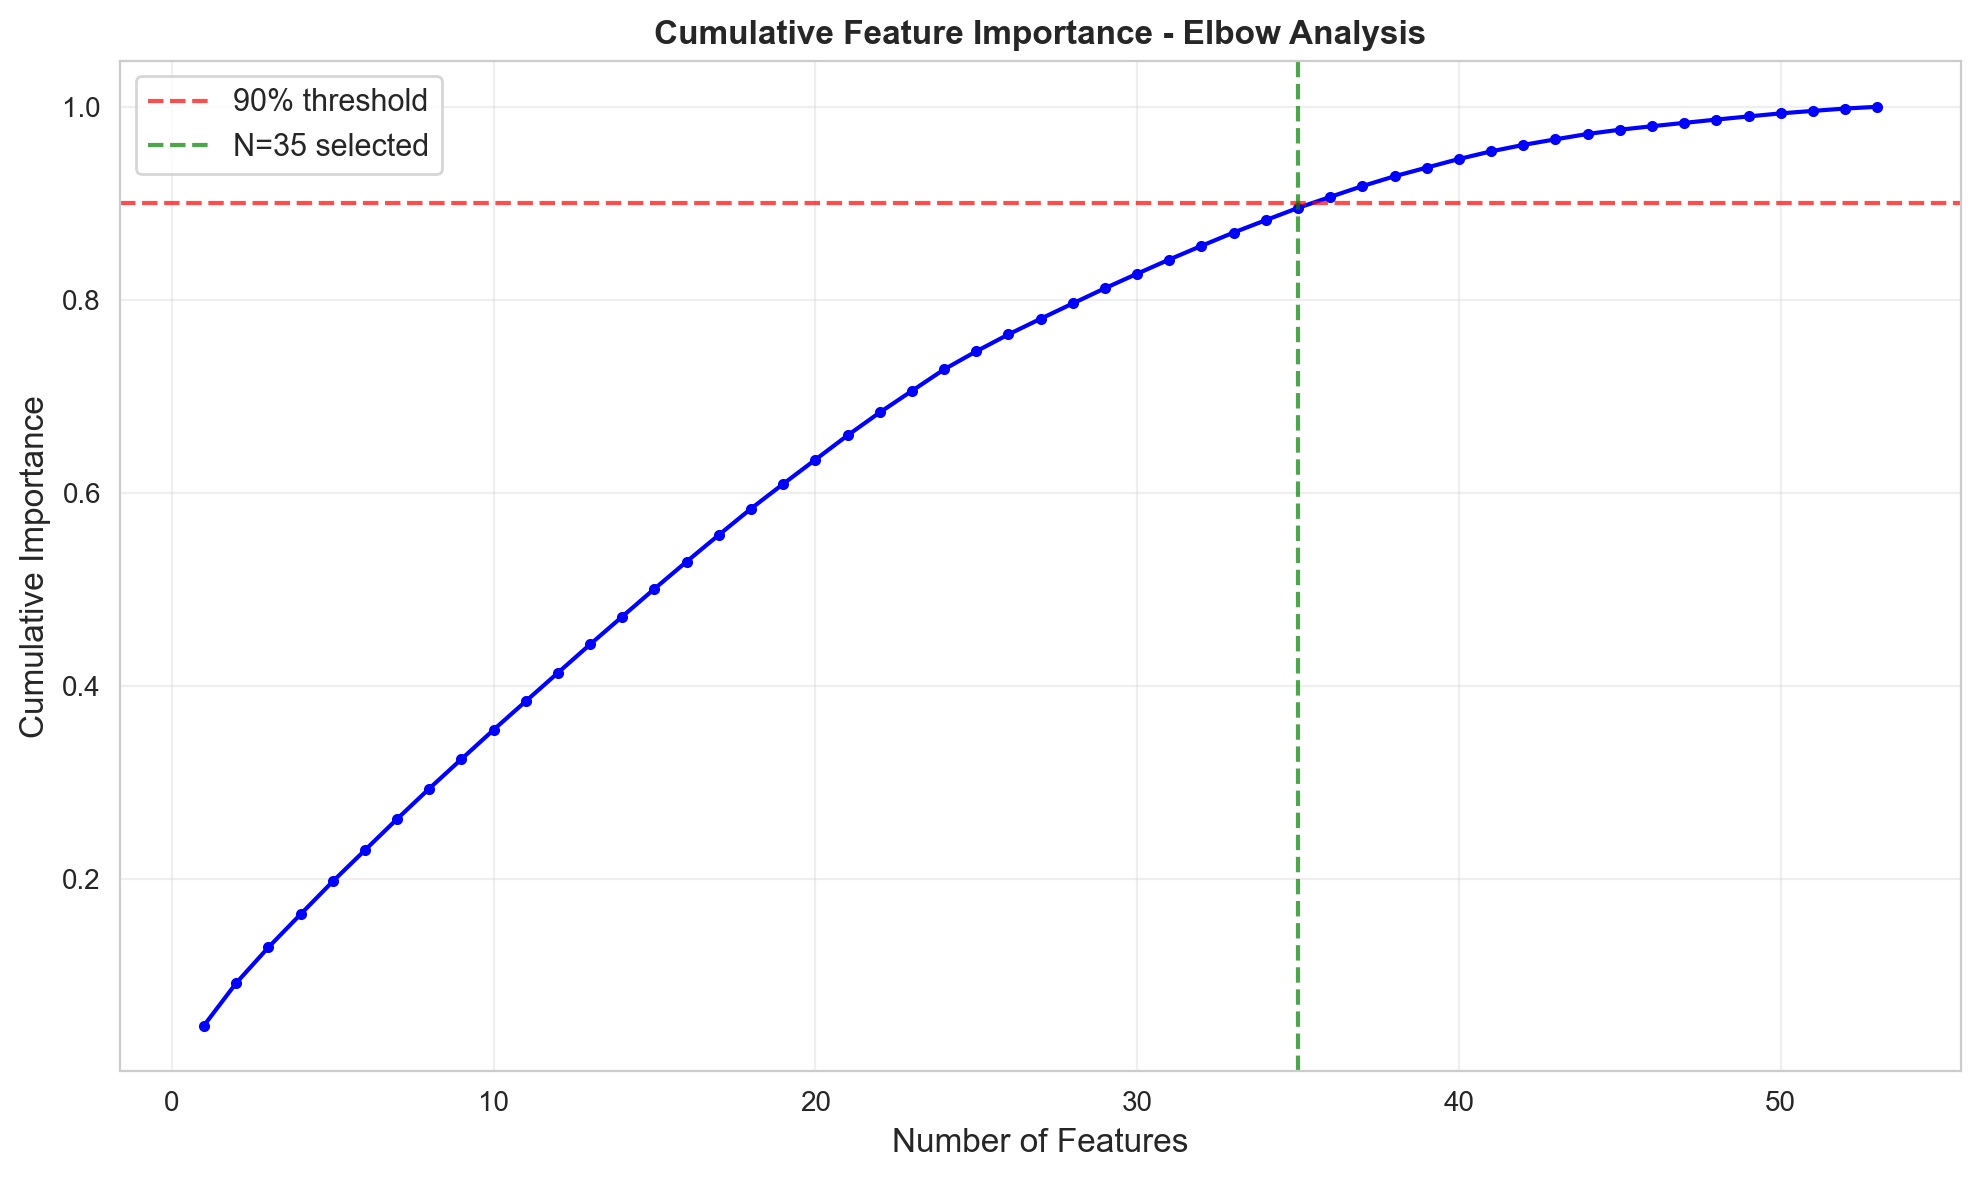
\includegraphics[width=0.78\textwidth]{figures/fig_cumulative_importance.png}
    \caption{Cumulative feature importance showing the 90\% threshold used for selection.}
    \label{fig:cumulative_importance}
\end{figure}

Permutation importance was also used as a validation step. This helped confirm that the final feature subset was not only important according to the training model itself, but also meaningful under feature-shuffling analysis \cite{biau2016rf}.

\begin{figure}[H]
    \centering
    
\includegraphics[width=0.78\textwidth]{figures/fig_importance_permutation.png}
    \caption{Permutation importance for the selected feature set, used as a robustness check for feature relevance.}
    \label{fig:perm_importance}
\end{figure}

\subsection{Dimensionality Reduction}
\textbf{After feature selection}, PCA and t-SNE were applied on the 29 selected features for exploratory visualization \cite{pearson1901pca,maaten2008tsne}. This ordering is intentional: important features were identified first, and dimensionality reduction was applied only to the already-reduced feature set.

PCA showed that the selected feature space still retained substantial complexity. Multiple principal components were needed to explain most of the variance, which suggests that the article attributes are distributed across several dimensions rather than concentrated in only a few dominant patterns.

\begin{figure}[H]
    \centering
    
\includegraphics[width=0.72\textwidth]{figures/fig_pca_variance.png}
    \caption{Explained variance plot for PCA on the selected features.}
    \label{fig:pca_variance}
\end{figure}

\begin{figure}[H]
    \centering
    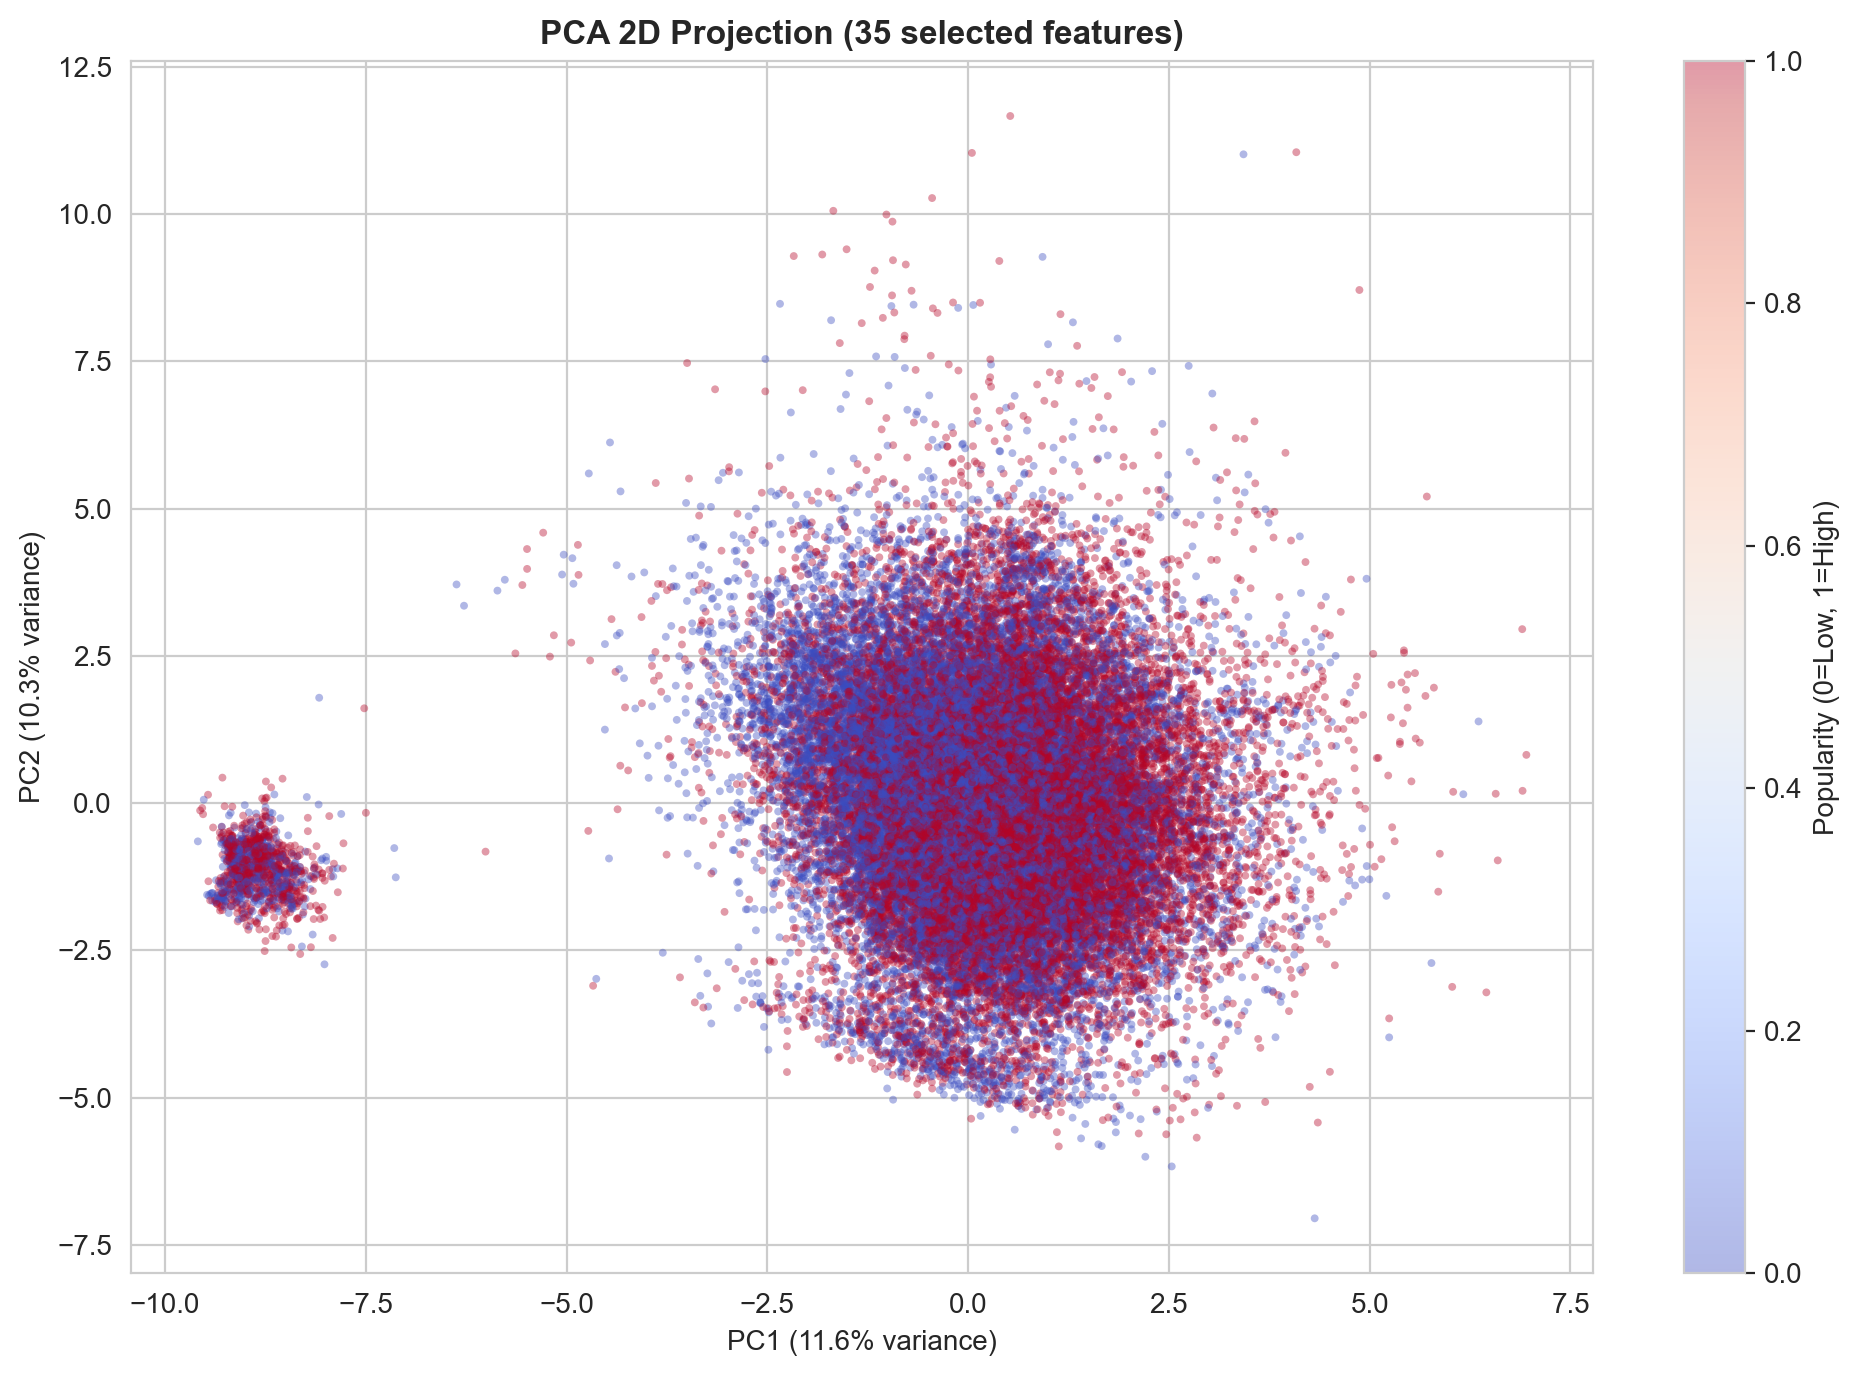
\includegraphics[width=0.72\textwidth]{figures/fig_pca_2d.png}
    \caption{Two-dimensional PCA projection of the selected feature space.}
    \label{fig:pca_2d}
\end{figure}

The t-SNE representation further suggested that the data contains local structure, but does not break into strongly separated global groups. This result is consistent with the clustering outcomes discussed later in the report.

\begin{figure}[H]
    \centering
    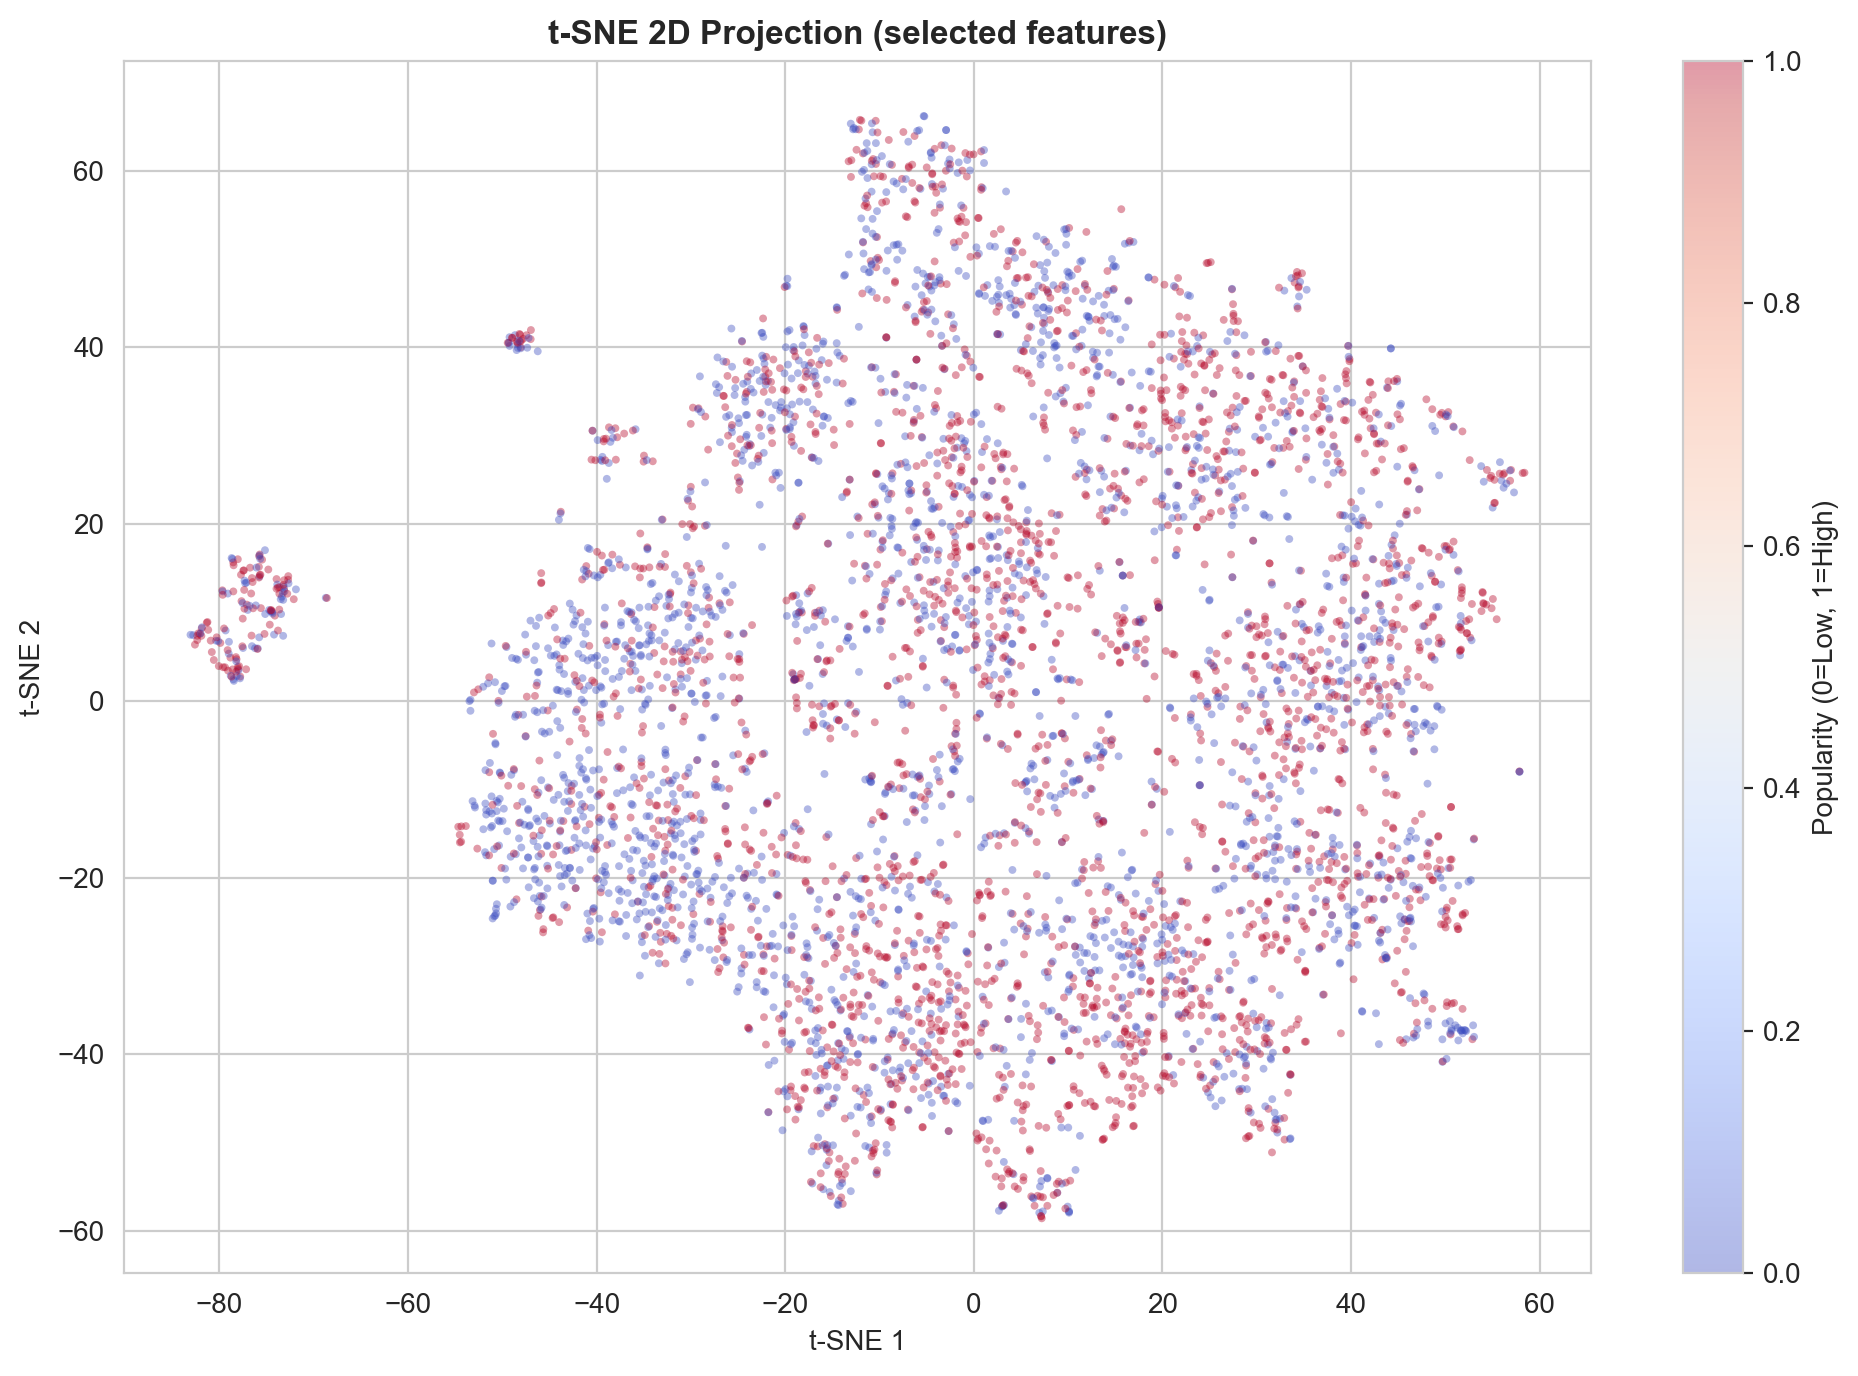
\includegraphics[width=0.72\textwidth]{figures/fig_tsne_2d.png}
    \caption{t-SNE projection of the selected feature space, showing overlap between local article groups.}
    \label{fig:tsne_2d}
\end{figure}

\section{Task-Oriented Methodology}

All supervised tasks share a common experimental setup to ensure reproducibility. The dataset was split into 80\% training and 20\% test sets using a fixed random seed of 42. For classification tasks, the split was stratified on the target label. Each task was evaluated under two conditions --- before preprocessing (imputed only) and after preprocessing (imputed + StandardScaler) --- as defined in Section~\ref{sec:preprocessing_definition}.

\subsection{Task 1: Predicting Whether a News Article Will Be Popular}
Task 1 is formulated as a supervised binary classification problem. The input consists of the 29 selected features, and the output is a binary label indicating whether an article is popular (shares $\geq$ 1400, the dataset median) or unpopular.

Eight classification models were evaluated:
\begin{enumerate}[leftmargin=1.5em]
    \item \textit{Linear:} Logistic Regression \cite{hosmer2013logistic}
    \item \textit{Distance-based:} K-Nearest Neighbors (KNN), Support Vector Machine (SVM)
    \item \textit{Tree-based ensembles:} Decision Tree, Random Forest \cite{breiman2001rf,biau2016rf}, Gradient Boosting, AdaBoost
    \item \textit{Probabilistic:} Naive Bayes
\end{enumerate}

Performance is assessed using accuracy, precision, recall, F1-score, and ROC-AUC. Models are grouped by family to identify which \textit{group} of models performs best overall.

\subsection{Task 2: Predicting the Number of Shares an Article Will Receive}
Task 2 is formulated as a supervised regression problem. The goal is to estimate article engagement using the transformed target $\log(1 + \texttt{shares})$. This transformation is applied because the original share counts are highly right-skewed with a long tail.

Seven regression models were evaluated:
\begin{enumerate}[leftmargin=1.5em]
    \item \textit{Linear:} Linear Regression, Ridge Regression \cite{montgomery2012linear,hoerl1970ridge}, Lasso Regression
    \item \textit{Tree-based ensembles:} Decision Tree Regressor, Random Forest Regressor \cite{breiman2001rf}, Gradient Boosting Regressor
    \item \textit{Distance-based:} Support Vector Regression (SVR)
\end{enumerate}

Performance is evaluated using RMSE (log and original scale), MAE (log scale), and $R^2$.

\subsection{Task 3: Discovering Natural Groupings of News Articles}
Task 3 is an unsupervised clustering task designed to explore whether articles form natural groups in the 29-feature space. All features were scaled using StandardScaler before clustering. Two methods were used:

\begin{itemize}[leftmargin=1.5em]
    \item \textbf{K-Means} \cite{macqueen1967kmeans}: tested for $k = 2, 3, \ldots, 10$ with $n\_init = 10$ and random seed 42. The optimal $k$ was selected using the highest silhouette score.
    \item \textbf{DBSCAN} \cite{ester1996dbscan}: run with $\epsilon = 3.0$ and $min\_samples = 10$ as a density-based alternative that can detect irregular cluster shapes and identify noise points.
\end{itemize}

Cluster quality is evaluated using silhouette scores, inertia (elbow method), and descriptive profiling of each detected group.

\subsection{Task 4: Identifying Content Patterns Associated with High Engagement}
Task 4 applies association rule mining to identify combinations of binary indicators that tend to occur in high-share articles. The analysis uses the dataset's 13 binary indicator columns (7 weekday flags and 6 channel flags) along with a binarized popularity target (shares $\geq$ median).

The Apriori algorithm \cite{agrawal1994association} is applied with adaptive minimum support ($\max(0.05, 50 / N)$ where $N$ is the number of rows), minimum confidence of 0.3, and minimum lift of 1.01 to filter out trivial rules. Rules are evaluated using support, confidence, and lift.

\subsection{Task 5: Optimizing Article Formatting and Media Usage for Maximum Reach}
Task 5 focuses on a smaller set of 6 structural article features: \texttt{n\_tokens\_title}, \texttt{n\_tokens\_content}, \texttt{num\_imgs}, \texttt{num\_videos}, \texttt{num\_hrefs}, and \texttt{num\_self\_hrefs}. The target is $\log(1 + \texttt{shares})$.

This task is approached as a focused regression problem using four models: Ridge Regression, Lasso Regression, Random Forest Regressor, and Gradient Boosting Regressor. In addition to model performance, the analysis examines model coefficients and feature importance scores to provide interpretable insights about how article formatting choices relate to engagement.

\subsection{Task 6: Recommending the Optimal Publication Window (Weekday vs.\ Weekend)}
Task 6 explores whether article content and tone can help distinguish weekday versus weekend publication behavior. This is framed as a binary classification problem where the output indicates weekday (0) or weekend (1).

The input consists of 26 features: 16 NLP/sentiment features (subjectivity, polarity, positive/negative word rates), 5 channel indicators, and 5 LDA topic features (\texttt{LDA\_00} through \texttt{LDA\_04}, which are Latent Dirichlet Allocation topic closeness scores pre-computed in the original dataset).

\textit{Note:} The dataset does not contain hour-level publication timestamps. Only binary weekday indicators (\texttt{weekday\_is\_monday} through \texttt{weekday\_is\_sunday}) and an \texttt{is\_weekend} flag are available. Therefore, this task uses weekday vs.\ weekend as the temporal dimension.

Four models are used: Logistic Regression, Random Forest, Gradient Boosting, and SVM. Performance is evaluated using accuracy, precision, recall, F1-score, and ROC-AUC. Because the weekend class represents only about 13\% of articles, the interpretation places strong emphasis on class imbalance and the limitations of using accuracy alone.

\subsection{Spark-Based Scalability Demonstration}
In addition to the six analytical tasks, a PySpark workflow is included as a scalability demonstration \cite{zaharia2016spark}. The pipeline consists of three stages:
\begin{enumerate}[leftmargin=1.5em]
    \item \textbf{VectorAssembler}: combines all feature columns into a single feature vector
    \item \textbf{StandardScaler}: normalizes features (with mean and standard deviation)
    \item \textbf{Random Forest Classifier}: trained with 100 trees and random seed 42
\end{enumerate}

The data was split 80/20 (seed 42) and the same median-based popularity threshold from Task~1 was used. The Spark results are compared with the scikit-learn Random Forest implementation to examine consistency and portability across frameworks.

\section{Results and Findings by Task}

This section presents the results obtained for each of the six defined tasks. For supervised
tasks, model performance is compared before and after preprocessing in order to evaluate the
impact of scaling and feature preparation. For exploratory tasks, the findings are presented
through clustering quality, association rules, and interpretable feature-based insights.

\subsection{Task 1: Predicting Whether a News Article Will Be Popular}

Task 1 was formulated as a binary classification problem, where an article was labeled as
\textit{popular} if its number of shares was greater than or equal to the median value
(1400), and \textit{unpopular} otherwise. Eight classification models were evaluated before and
after preprocessing.

\subsubsection*{Results Before Preprocessing}

\begin{table}[H]
\centering
\caption{Task 1 classification results before preprocessing}
\begin{tabular}{lccccc}
\toprule
Model & Accuracy & Precision & Recall & F1 & ROC-AUC \\
\midrule
Logistic Regression & 0.5970 & 0.6113 & 0.6724 & 0.6404 & 0.6318 \\
KNN & 0.5591 & 0.5870 & 0.5861 & 0.5866 & 0.5785 \\
SVM & 0.5055 & 0.5235 & 0.8152 & 0.6376 & 0.4507 \\
Decision Tree & 0.5654 & 0.5941 & 0.5859 & 0.5900 & 0.5639 \\
Random Forest & 0.6412 & 0.6531 & 0.6987 & 0.6751 & 0.6919 \\
Gradient Boosting & 0.6483 & 0.6566 & 0.7145 & 0.6843 & 0.7015 \\
AdaBoost & 0.6379 & 0.6483 & 0.7024 & 0.6743 & 0.6916 \\
Naive Bayes & 0.5176 & 0.6750 & 0.1851 & 0.2905 & 0.6208 \\
\bottomrule
\end{tabular}
\end{table}

\subsubsection*{Results After Preprocessing}

\begin{table}[H]
\centering
\caption{Task 1 classification results after preprocessing}
\begin{tabular}{lccccc}
\toprule
Model & Accuracy & Precision & Recall & F1 & ROC-AUC \\
\midrule
Logistic Regression & 0.6305 & 0.6412 & 0.6982 & 0.6685 & 0.6762 \\
KNN & 0.5871 & 0.6181 & 0.5918 & 0.6047 & 0.6111 \\
SVM & 0.5457 & 0.5862 & 0.5053 & 0.5428 & 0.5584 \\
Decision Tree & 0.5639 & 0.5921 & 0.5871 & 0.5896 & 0.5622 \\
Random Forest & 0.6409 & 0.6526 & 0.6996 & 0.6753 & 0.6926 \\
Gradient Boosting & 0.6469 & 0.6554 & 0.7133 & 0.6831 & 0.7016 \\
AdaBoost & 0.6379 & 0.6483 & 0.7024 & 0.6743 & 0.6916 \\
Naive Bayes & 0.5013 & 0.6716 & 0.1281 & 0.2152 & 0.6354 \\
\bottomrule
\end{tabular}
\end{table}

The best model before preprocessing was Gradient Boosting with an accuracy of 0.6483, and the
best model after preprocessing was again Gradient Boosting with an accuracy of 0.6469. Grouping models by family reveals a clear hierarchy:
\begin{itemize}[leftmargin=1.5em]
    \item \textbf{Tree-based ensembles} (RF, GB, AdaBoost): strongest group, accuracy 0.64--0.65
    \item \textbf{Linear models} (Logistic Regression): moderate, improved by scaling (0.60 $\to$ 0.63)
    \item \textbf{Distance-based} (KNN, SVM): weakest, most sensitive to feature scaling
    \item \textbf{Probabilistic} (Naive Bayes): poor recall due to violated independence assumptions
\end{itemize}
Preprocessing improved scale-sensitive models (Logistic Regression: +3.4\%, KNN: +2.8\%) but had negligible effect on tree-based ensembles, which are inherently scale-invariant.

\begin{figure}[H]
    \centering
    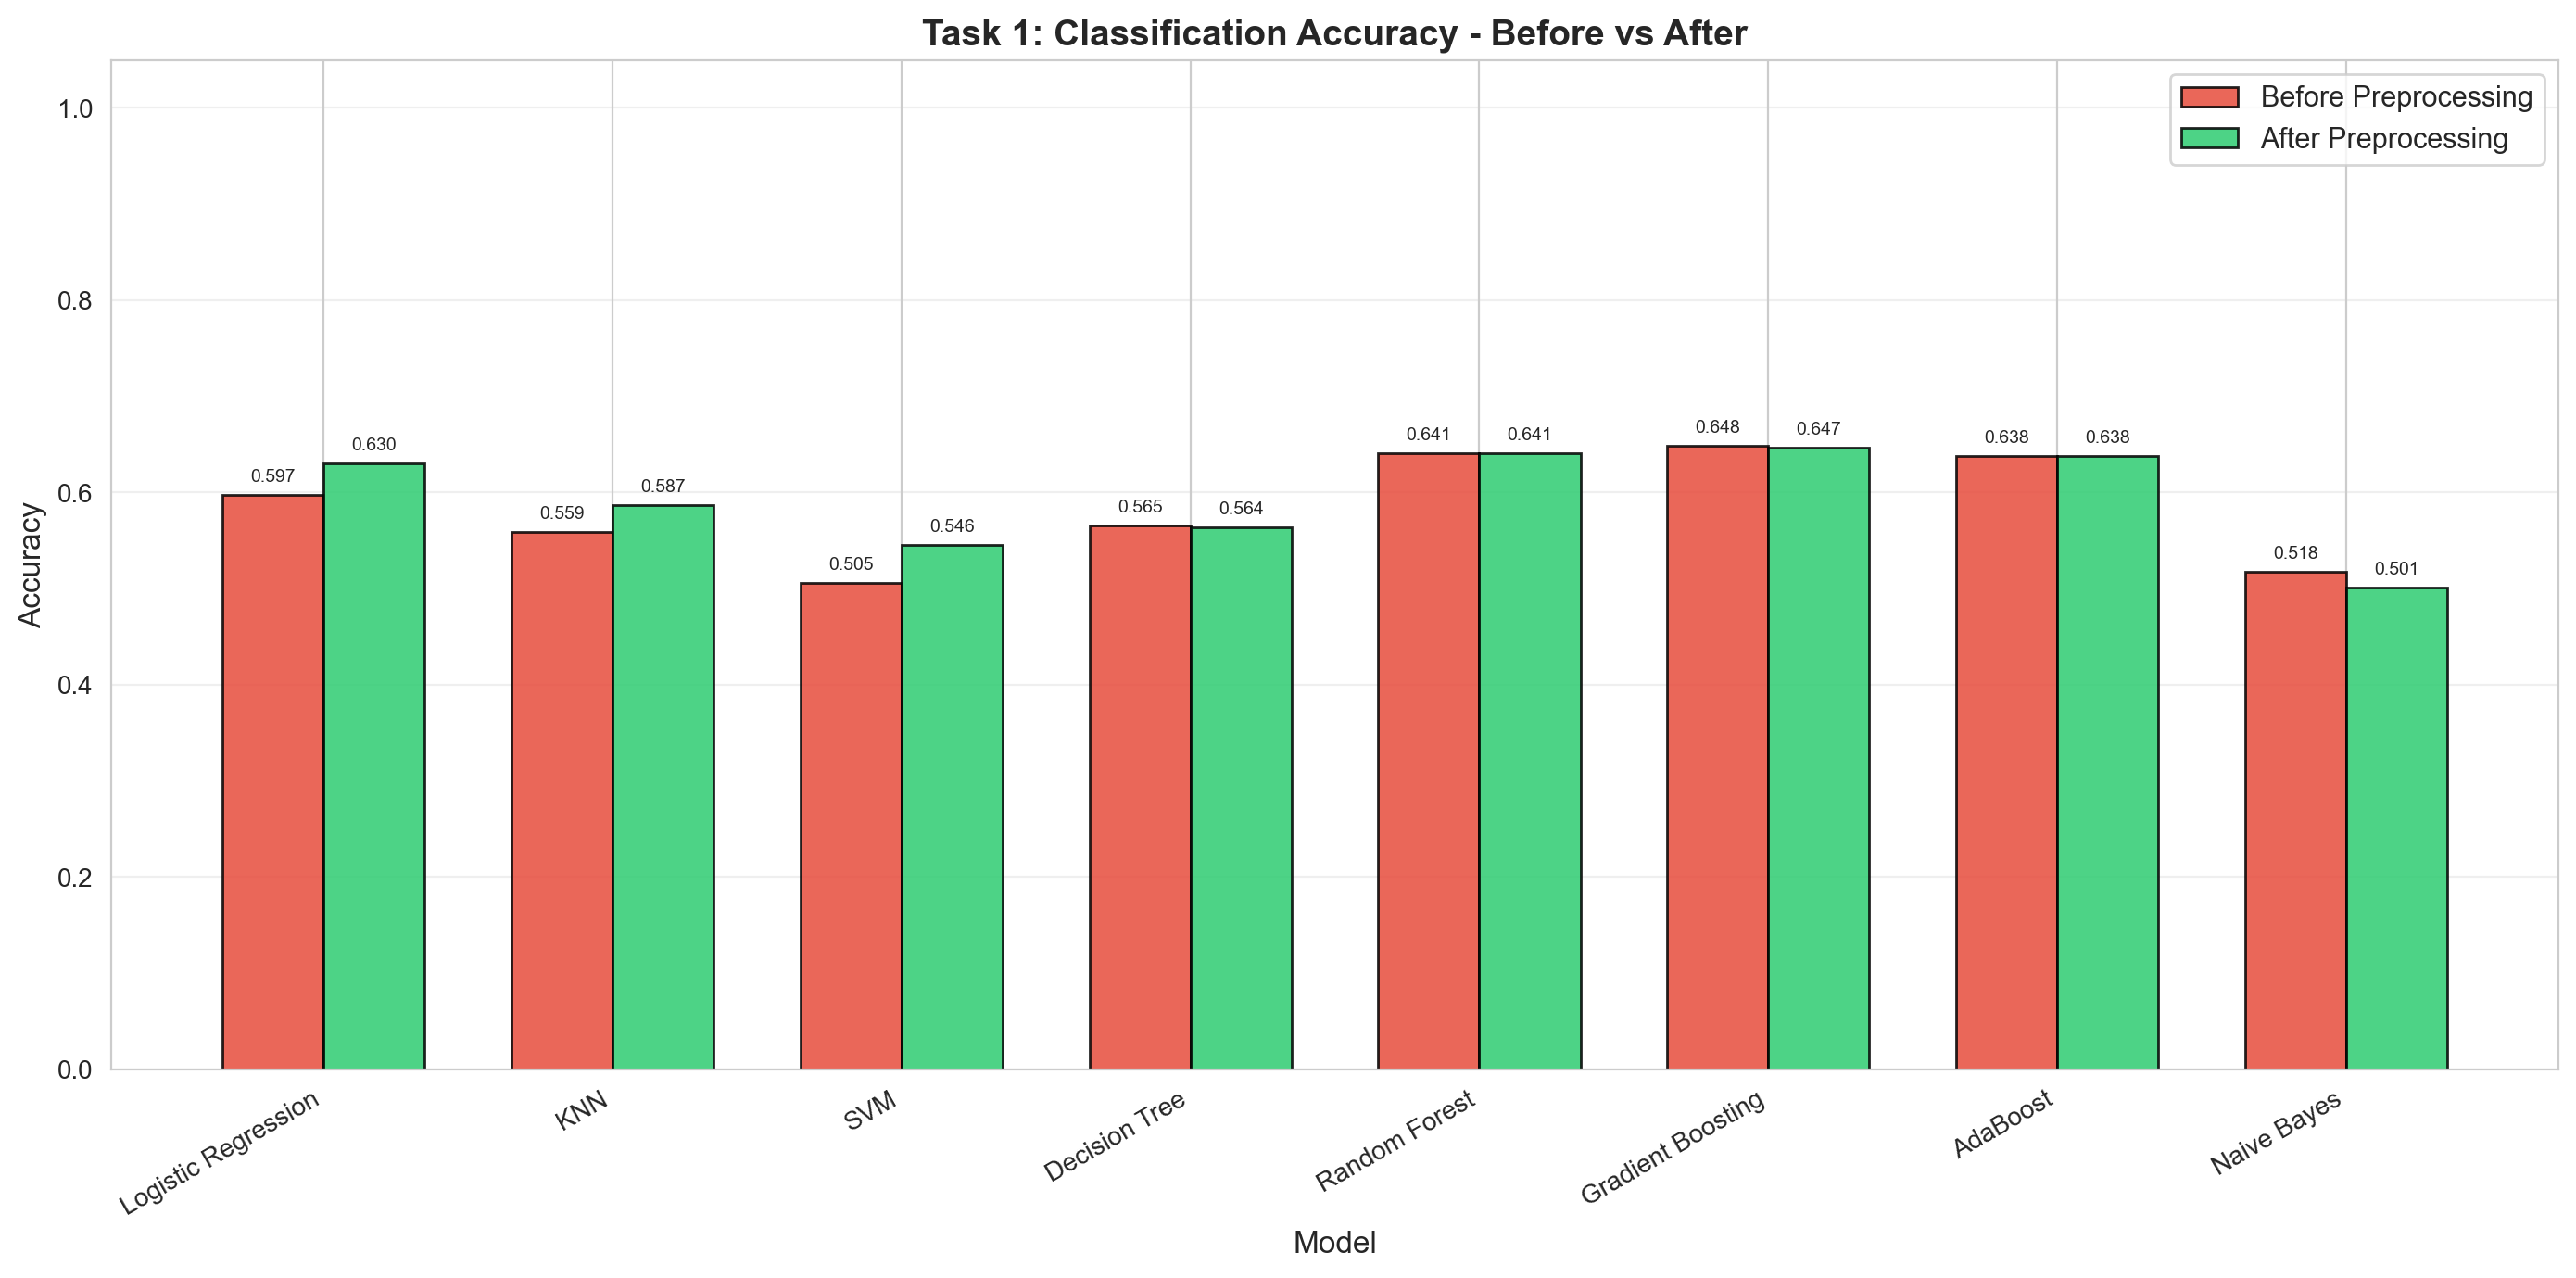
\includegraphics[width=0.7\textwidth]{figures/fig_task1_accuracy_comparison.png}
    \caption{Accuracy comparison for Task 1 classification models.}
\end{figure}

\begin{figure}[H]
    \centering
    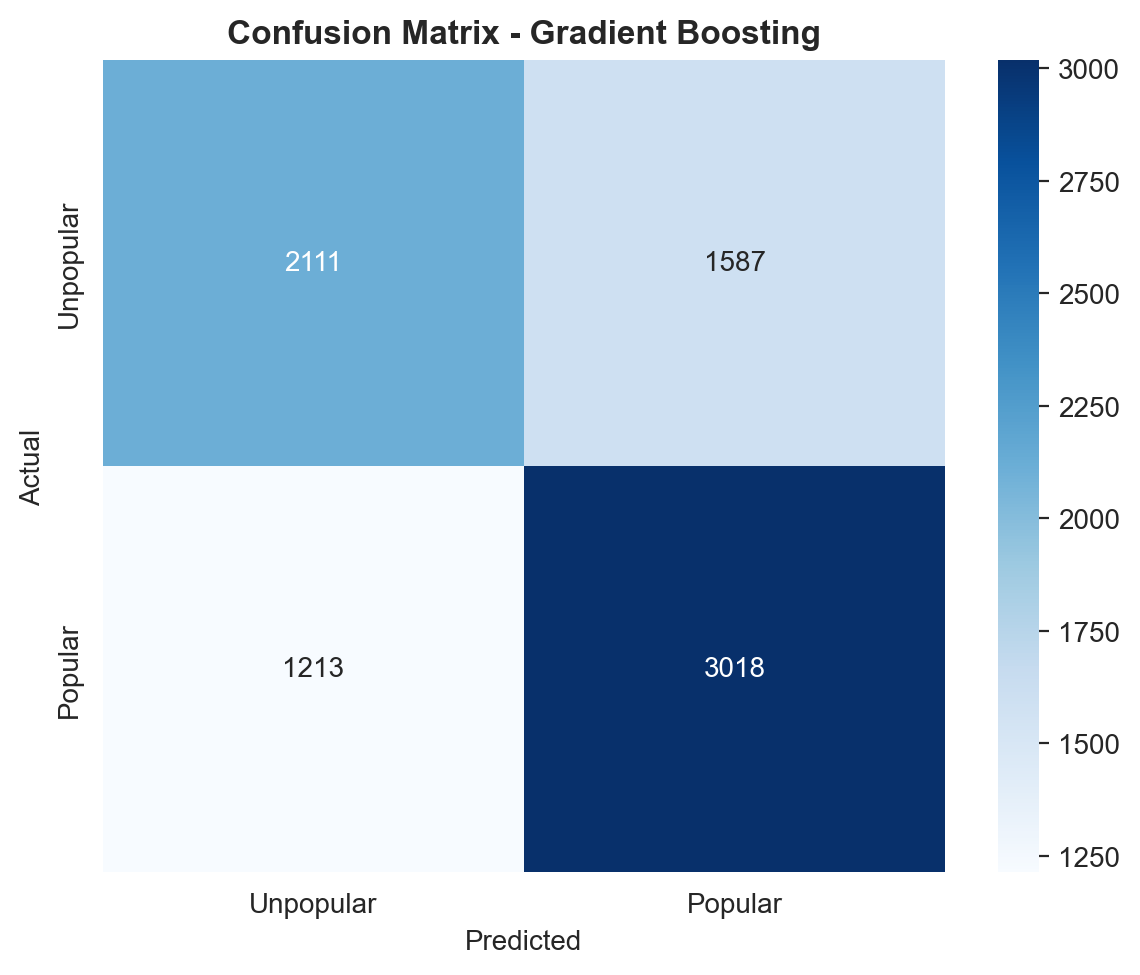
\includegraphics[width=0.65\textwidth]{figures/fig_task1_cm_best.png}
    \caption{Confusion matrix for the best Task 1 model.}
\end{figure}

\FloatBarrier

\subsection{Task 2: Predicting the Number of Shares an Article Will Receive}

Task 2 was formulated as a regression problem using the transformed target variable
$\log(1+\text{shares})$. Seven regression models were evaluated before and after preprocessing.

\subsubsection*{Results Before Preprocessing}

\begin{table}[H]
\centering
\caption{Task 2 regression results before preprocessing}
\begin{tabular}{lcccc}
\toprule
Model & RMSE$_{\log}$ & MAE$_{\log}$ & $R^2$ & RMSE$_{\text{orig}}$ \\
\midrule
Linear Regression & 0.8856 & 0.6574 & 0.1015 & 14646.95 \\
Ridge Regression & 0.8855 & 0.6573 & 0.1018 & 14646.83 \\
Lasso Regression & 0.8899 & 0.6636 & 0.0928 & 14652.19 \\
Decision Tree Regressor & 1.2644 & 0.9382 & -0.8314 & 18959.64 \\
Random Forest Regressor & 0.8727 & 0.6493 & 0.1275 & 14613.66 \\
Gradient Boosting Regressor & 0.8680 & 0.6408 & 0.1369 & 14631.04 \\
SVR & 2.6864 & 2.5036 & -7.2670 & 14994.45 \\
\bottomrule
\end{tabular}
\end{table}

\subsubsection*{Results After Preprocessing}

\begin{table}[H]
\centering
\caption{Task 2 regression results after preprocessing}
\begin{tabular}{lcccc}
\toprule
Model & RMSE$_{\log}$ & MAE$_{\log}$ & $R^2$ & RMSE$_{\text{orig}}$ \\
\midrule
Linear Regression & 0.8856 & 0.6574 & 0.1015 & 14646.95 \\
Ridge Regression & 0.8856 & 0.6574 & 0.1015 & 14646.87 \\
Lasso Regression & 0.8879 & 0.6616 & 0.0969 & 14657.53 \\
Decision Tree Regressor & 1.2673 & 0.9438 & -0.8397 & 18589.44 \\
Random Forest Regressor & 0.8731 & 0.6499 & 0.1267 & 14613.30 \\
Gradient Boosting Regressor & 0.8680 & 0.6411 & 0.1370 & 14630.31 \\
SVR & 0.9420 & 0.6733 & -0.0166 & 14690.96 \\
\bottomrule
\end{tabular}
\end{table}

Gradient Boosting Regressor achieved the best performance both before and after preprocessing,
with $R^2$ values of 0.1369 and 0.1370 respectively. As with Task~1, tree-based ensembles
(RF: $R^2 = 0.13$, GB: $R^2 = 0.14$) outperformed linear models ($R^2 \approx 0.10$), while
distance-based methods (SVR: $R^2 < 0$ before scaling) performed worst.

The low $R^2$ values are consistent with published research on this dataset --- Stanford CS229
projects on the same UCI data reported $R^2$ values of approximately 10\%. This reflects the
inherent difficulty of predicting social media shares from content features alone, where external
factors (viral network effects, current events, platform algorithms) account for the majority of
the variance in engagement.

\begin{figure}[H]
    \centering
    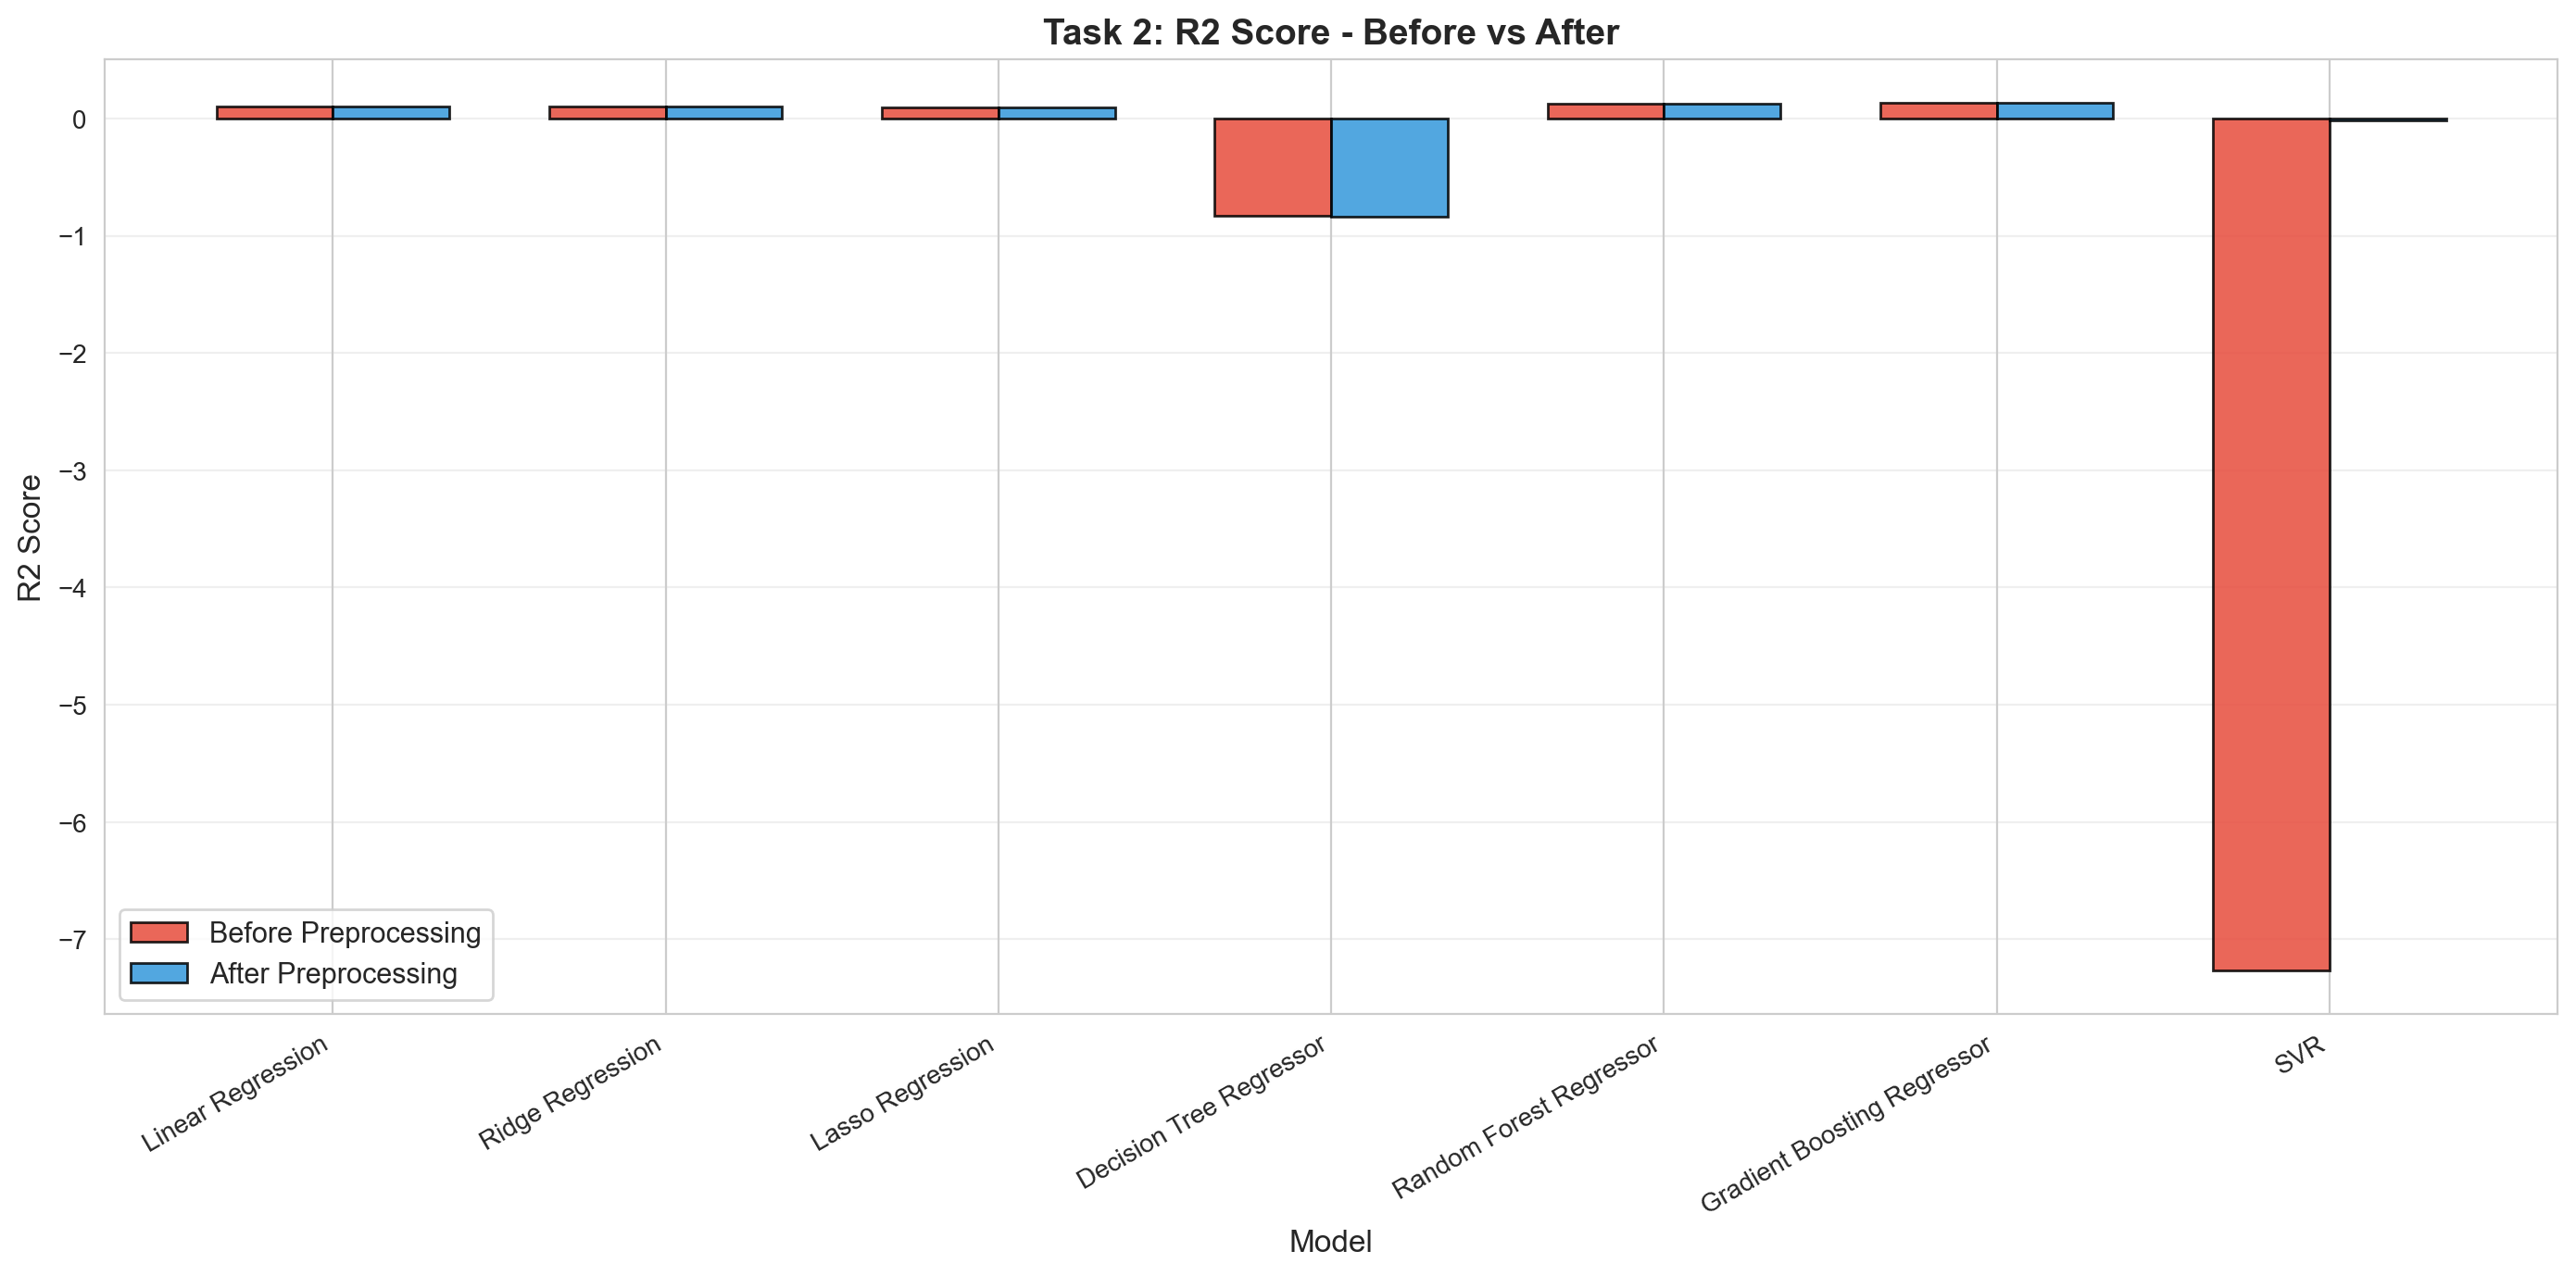
\includegraphics[width=0.7\textwidth]{figures/fig_task2_r2_comparison.png}
    \caption{$R^2$ comparison for Task 2 regression models.}
\end{figure}

\begin{figure}[H]
    \centering
    
\includegraphics[width=0.65\textwidth]{figures/fig_task2_pred_vs_actual.png}
    \caption{Predicted versus actual values for the best Task 2 model.}
\end{figure}

\FloatBarrier

\subsection{Task 3: Discovering Natural Groupings of News Articles}

Task 3 explored whether the dataset contains natural clusters of articles based on the selected
features. K-Means and DBSCAN were applied and evaluated primarily using the silhouette score.

The elbow method was first used to assess candidate values of $k$ for K-Means. The highest
silhouette score was obtained for $k=2$, where K-Means achieved a silhouette score of 0.4067.
Cluster profiling showed one dominant cluster containing most of the articles and one much
smaller subgroup with stronger topic and keyword-related characteristics.

DBSCAN identified 11 clusters and 9741 noise points, but produced a much lower silhouette
score of 0.0359 when noise points were excluded. This indicates that DBSCAN was less effective
for this dataset.

Overall, K-Means performed better than DBSCAN, but the clustering results suggest that the
dataset does not contain strongly separated natural article groups. Instead, article characteristics
appear to vary more continuously across the feature space.

\begin{figure}[H]
    \centering
    
\includegraphics[width=0.62\textwidth]{figures/fig_task3_clustering_elbow.png}
    \caption{Elbow analysis for Task 3 clustering.}
\end{figure}

\begin{figure}[H]
    \centering
    
\includegraphics[width=0.62\textwidth]{figures/fig_task3_kmeans_clusters.png}
    \caption{K-Means clustering result for Task 3.}
\end{figure}

\begin{figure}[H]
    \centering
    
\includegraphics[width=0.62\textwidth]{figures/fig_task3_dbscan_clusters.png}
    \caption{DBSCAN clustering result for Task 3.}
\end{figure}

\FloatBarrier

\subsection{Task 4: Identifying Content Patterns Associated with High Engagement}

Task 4 used association rule mining to identify feature combinations that tend to appear in
high-share articles. Using binary indicators and a binarized target variable, the Apriori algorithm
produced 27 frequent itemsets and 7 rules with lift greater than 1.01.

Among the most meaningful rules, weekend publication, technology channel membership, and
Friday publication showed positive association with high-share outcomes. In particular, the rule
\textit{is\_weekend $\Rightarrow$ shares\_high} achieved confidence 0.7146 and lift 1.3393,
showing a noticeably higher likelihood of popularity for weekend articles.

Although some rules were trivial due to the structure of binary weekday indicators, the
non-trivial rules still provided useful insights into content characteristics associated with stronger
engagement.

\begin{figure}[H]
    \centering
    
\includegraphics[width=0.68\textwidth]{figures/fig_task4_association_rules.png}
    \caption{Association rule mining results for Task 4.}
\end{figure}

\FloatBarrier

\subsection{Task 5: Optimizing Article Formatting and Media Usage for Maximum Reach}

Task 5 focused on a smaller set of structural article features:
\textit{n\_tokens\_title}, \textit{n\_tokens\_content}, \textit{num\_imgs},
\textit{num\_videos}, \textit{num\_hrefs}, and \textit{num\_self\_hrefs}.
The goal was to understand how article formatting and media usage relate to shares.

\begin{table}[H]
\centering
\caption{Task 5 regression results using structural formatting features}
\begin{tabular}{lcccc}
\toprule
Model & RMSE$_{\log}$ & MAE$_{\log}$ & $R^2$ & RMSE$_{\text{orig}}$ \\
\midrule
Ridge Regression & 0.9171 & 0.7011 & 0.0189 & 11080.36 \\
Lasso Regression & 0.9177 & 0.7011 & 0.0176 & 11083.98 \\
Random Forest Regressor & 0.9417 & 0.7261 & -0.0346 & 11042.59 \\
Gradient Boosting Regressor & 0.8981 & 0.6867 & 0.0591 & 11047.83 \\
\bottomrule
\end{tabular}
\end{table}

The relatively low $R^2$ values show that formatting variables alone explain only a limited part
of the variation in shares. However, the coefficient-based and feature-importance analyses still
provided useful directional insights. Links and images showed positive associations with higher
engagement, while title length and self-references showed weaker or negative associations in some
models.

These results suggest that formatting and media usage matter, but they are not sufficient by
themselves to fully explain article popularity.

\begin{figure}[H]
    \centering
    
\includegraphics[width=0.68\textwidth]{figures/fig_task5_feature_importance.png}
    \caption{Feature importance for Task 5 formatting analysis.}
\end{figure}

\FloatBarrier

\subsection{Task 6: Recommending the Optimal Publication Window}

Task 6 investigated whether content, sentiment, and topic-related features could help distinguish
between weekday and weekend publication patterns. This was treated as a binary classification
task.

\subsubsection*{Results Before Preprocessing}

\begin{table}[H]
\centering
\caption{Task 6 publication window results before preprocessing}
\begin{tabular}{lccccc}
\toprule
Model & Accuracy & Precision & Recall & F1 & ROC-AUC \\
\midrule
Logistic Regression & 0.8691 & 0.0000 & 0.0000 & 0.0000 & 0.5514 \\
Random Forest & 0.8716 & 0.7174 & 0.0318 & 0.0609 & 0.6022 \\
Gradient Boosting & 0.8700 & 0.6296 & 0.0164 & 0.0319 & 0.6260 \\
SVM & 0.8691 & 0.0000 & 0.0000 & 0.0000 & 0.5368 \\
\bottomrule
\end{tabular}
\end{table}

\subsubsection*{Results After Preprocessing}

\begin{table}[H]
\centering
\caption{Task 6 publication window results after preprocessing}
\begin{tabular}{lccccc}
\toprule
Model & Accuracy & Precision & Recall & F1 & ROC-AUC \\
\midrule
Logistic Regression & 0.8691 & 0.0000 & 0.0000 & 0.0000 & 0.5545 \\
Random Forest & 0.8720 & 0.7255 & 0.0356 & 0.0680 & 0.6203 \\
Gradient Boosting & 0.8700 & 0.6296 & 0.0164 & 0.0319 & 0.6251 \\
SVM & 0.8702 & 1.0000 & 0.0087 & 0.0172 & 0.5646 \\
\bottomrule
\end{tabular}
\end{table}

Random Forest performed best on this task with an accuracy of 0.8720 after preprocessing.
However, this result should be interpreted carefully because the dataset is highly imbalanced
between weekday and weekend articles. The very low recall values for the weekend class indicate
that the models struggled to identify weekend articles reliably. Therefore, this task is more
appropriately treated as an exploratory investigation than as a strong recommendation model.

\begin{figure}[H]
    \centering
    
\includegraphics[width=0.68\textwidth]{figures/fig_task6_roc.png}
    \caption{ROC curve for Task 6 publication window classification.}
\end{figure}

\begin{figure}[H]
    \centering
    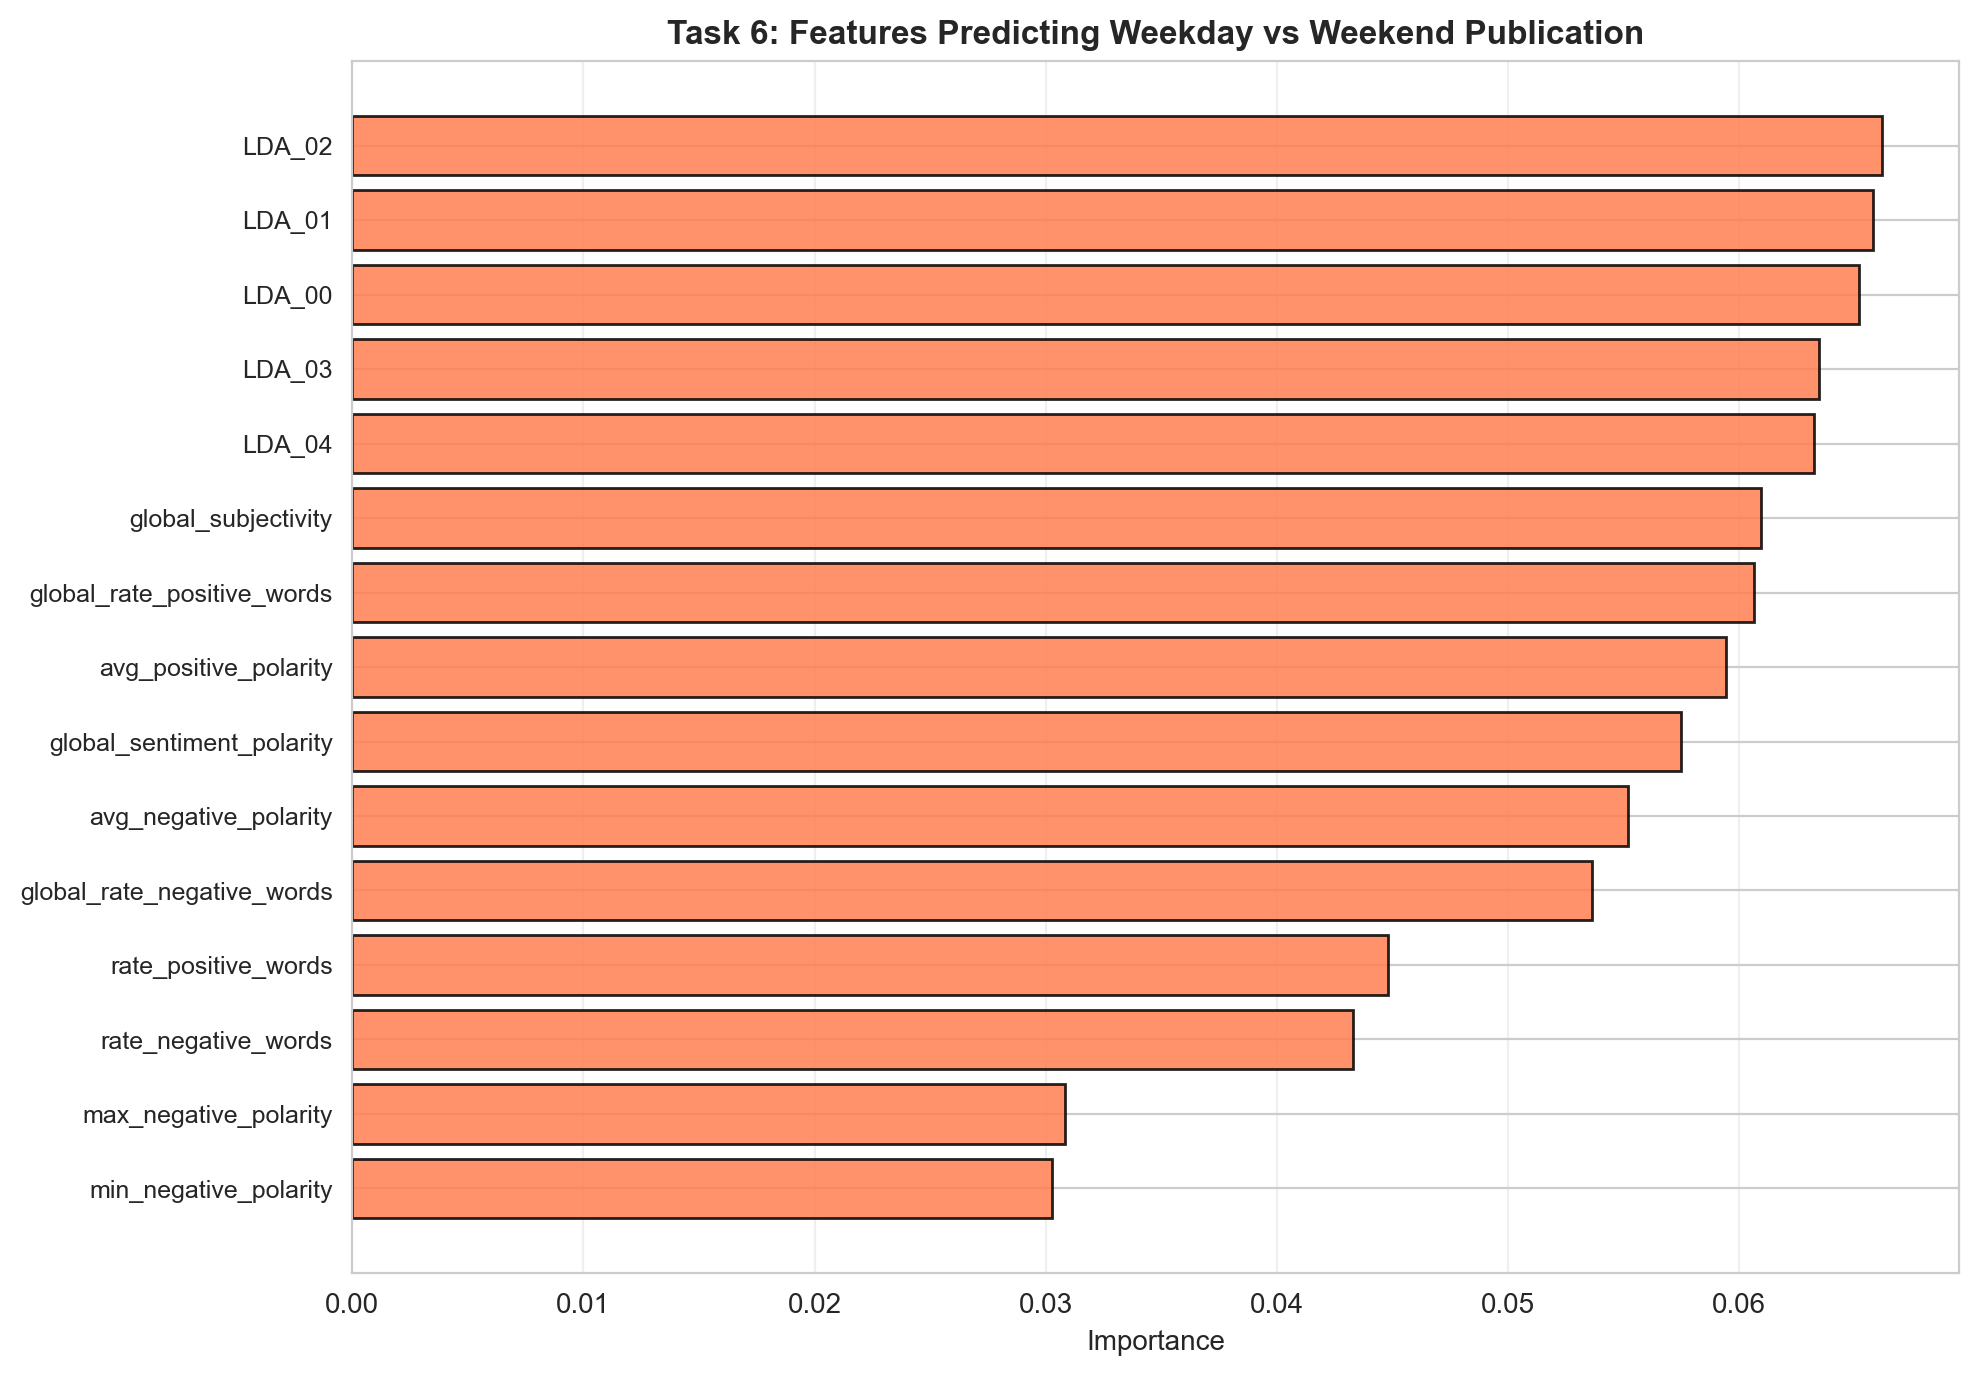
\includegraphics[width=0.68\textwidth]{figures/fig_task6_feature_importance.png}
    \caption{Feature importance for Task 6.}
\end{figure}

\FloatBarrier

\subsection{Scalability Demonstration with Spark}

In addition to the six analytical tasks, a Spark-based scalability demonstration was performed
to show how the workflow can be extended to distributed environments. A Spark Random Forest
classifier was trained using the same popularity threshold as Task 1.

The Spark model achieved an accuracy of 0.6539 and a ROC-AUC of 0.7087, which are very
close to the corresponding scikit-learn Random Forest results. This shows that the analytical
pipeline can be transferred to a distributed framework while maintaining comparable predictive
performance.

The demonstration shows how the same workflow could be scaled to much larger article datasets in future work.
\section{Discussion}

\subsection{Model Group Comparison}

Across Tasks 1 and 2, a clear pattern emerged in how different model families performed. This comparison addresses the professor's feedback to identify not just the best single model, but the best \textit{group} of models.

\begin{table}[H]
\centering
\caption{Model group performance summary across supervised tasks}
\begin{tabular}{llcc}
\toprule
\textbf{Model Group} & \textbf{Models} & \textbf{Task 1 Acc.} & \textbf{Task 2 $R^2$} \\
\midrule
Tree-based ensembles & RF, GB, AdaBoost & 0.64--0.65 & 0.13--0.14 \\
Linear models & LogReg, Ridge, Lasso & 0.60--0.63 & 0.09--0.10 \\
Distance-based & KNN, SVM, SVR & 0.51--0.59 & $<$0 to $-$7.27 \\
Probabilistic & Naive Bayes & 0.50--0.52 & --- \\
\bottomrule
\end{tabular}
\end{table}

\noindent \textbf{Tree-based ensembles} (Random Forest, Gradient Boosting, AdaBoost) consistently outperformed all other model families. This indicates that article popularity is shaped by non-linear feature interactions that tree-based methods capture well \cite{breiman2001rf,biau2016rf}. \textbf{Linear models} provided a moderate baseline and benefited most from preprocessing (scaling). \textbf{Distance-based models} (KNN, SVM, SVR) were the weakest, particularly SVR which produced negative $R^2$ values before scaling, indicating sensitivity to feature magnitudes and the high-dimensional feature space. Naive Bayes performed poorly due to its independence assumption being violated by the correlated feature set.

\subsection{Role of Preprocessing}

Preprocessing (StandardScaler) had a differential impact depending on model type. Scale-sensitive models such as Logistic Regression, KNN, and SVM showed meaningful improvement after scaling. In contrast, tree-based models (Gradient Boosting, Random Forest) showed negligible changes because they are scale-invariant --- they split on feature thresholds regardless of magnitude. The slight accuracy decrease for Gradient Boosting after preprocessing (0.6483 to 0.6469) is expected and reflects minor floating-point shifts in split boundaries rather than a meaningful degradation.

\subsection{Feature Engineering Impact}

The preliminary feature selection stage improved both the organization and interpretability of the project by focusing the analysis on 29 informative variables selected through a data-driven process. Keyword statistics (\texttt{kw\_max\_avg}, \texttt{kw\_avg\_max}), self-reference measures, LDA topic probabilities, and sentiment-related features appeared repeatedly as the most important factors, indicating that article popularity depends on a mix of topic relevance, language characteristics, and prior contextual signals.

\subsection{Exploratory Task Findings}

The exploratory tasks provided useful support, even when their results were not especially strong in a predictive sense. Clustering showed that the dataset does not naturally separate into sharply distinct article types, which helps explain why supervised models are more suitable for this problem. The selection of $k=2$ as the optimal cluster count aligns with the binary popular/unpopular split used in Task~1, suggesting that this is the most natural division in the data. Association rule mining reinforced the idea that timing and topic matter, but also showed that only a limited number of rules lead to meaningful engagement-related interpretation.

Task 5 added a practical layer to the project by isolating article formatting and media usage. While these structural variables alone had limited explanatory power ($R^2 \approx 0.06$ at best), they still offered useful directional insight into how article design may relate to engagement. This supports the idea that share performance is influenced not only by what an article is about, but also by how it is presented.

Task 6 was the weakest task in the project, largely because of class imbalance (only 13\% of articles were published on weekends) and weak weekend recall. However, including it still adds value because it shows an honest boundary of what the data can and cannot support. In a complete analytics project, reporting a weak result is often as important as reporting a strong one.

\subsection{Interpretation of Low $R^2$ in Task 2}

The best $R^2$ value of 0.137 may appear low but is consistent with published research on this exact dataset. Stanford CS229 projects by Ren \& Yang (2015) and Johnson \& Weinberger (2016) reported similar $R^2$ values of approximately 10\% on the same UCI Mashable data. Predicting social media shares is fundamentally a human behavior problem where external factors (viral network effects, current events, platform algorithms) account for the majority of variance. In social science domains, $R^2$ values of 10--15\% are generally accepted when the predictors capture only content-level features.

\subsection{Overall Structure}

Overall, the report shows that a task-oriented structure provides a clearer and more meaningful way to present the project. Instead of appearing as a sequence of unrelated techniques, the analysis becomes a connected study built around real analytical questions \cite{bishop2006prml,han2011datamining}.

\section{Challenges Faced}

Several challenges were encountered during the project.

First, the target variable \texttt{shares} was highly skewed, with a small number of articles receiving extremely high engagement. This made regression especially difficult and required the use of a log transformation to stabilize the target distribution.

Second, the original feature space contained a number of correlated variables, particularly among keyword-related and self-reference features. This required careful feature selection to reduce redundancy without discarding too much information.

Third, not all analytical tasks were equally strong. Some tasks, such as classification and regression, produced meaningful results, while others, such as clustering and publication timing prediction, showed weaker structure and required more cautious interpretation.

A further challenge was balancing practical interpretability with predictive performance. Models such as Gradient Boosting and Random Forest performed better, but simpler models were still necessary for comparison and interpretation.

Finally, the project required restructuring from a method-centered workflow into a task-oriented one. This created a more coherent report, but also required the analytical pipeline and the report narrative to be aligned carefully.

\section{Limitations}

This study has several limitations that should be acknowledged.

First, the dataset contains only the numerical article descriptors provided in the Online News Popularity dataset. It does not include the full article text, reader demographics, current events context, or platform-specific social dynamics, all of which may influence article engagement.

Second, the predictive performance of the regression task remains modest. This suggests that exact share counts are affected by substantial noise and external factors that are not captured in the available features.

Third, the clustering and association rule tasks provided limited evidence of strong underlying structure. While they contributed exploratory insight, they should not be interpreted as definitive segmentation or causal pattern discovery.

Finally, the publication timing task was heavily affected by class imbalance. Because weekend articles form a much smaller portion of the dataset, the classification results for this task are weak from a practical recommendation standpoint.


\section{Future Work}

Several directions could extend this project in meaningful ways.

First, for interpretability, future studies could apply SHAP (SHapley Additive exPlanations) values or partial dependence analysis more extensively to better explain how individual features influence model predictions at the instance level.

Second, the feature engineering pipeline could be improved by incorporating text-based features extracted directly from article content (e.g., TF-IDF, word embeddings), which are not available in the current dataset but could provide stronger predictive signals.

Third, the class imbalance issue in Task~6 could be addressed using techniques such as SMOTE (Synthetic Minority Oversampling), class-weighted models, or alternative evaluation metrics such as balanced accuracy.

Finally, the Spark pipeline could be extended to larger datasets or deployed in a multi-node cluster setting to evaluate performance, scalability, and distributed training behavior under true big-data conditions.

\section{Conclusion}

This project examined online news popularity through a task-oriented data analytics framework. Rather than presenting the work as a collection of methods, the report organized the analysis around six specific tasks: popularity classification, share prediction, article grouping, engagement pattern discovery, formatting analysis, and publication timing investigation. This structure made the project objectives clearer and connected the technical analysis to practical questions about article engagement.

The strongest results came from the supervised tasks, where ensemble models such as Gradient Boosting and Random Forest consistently outperformed simpler alternatives. Feature engineering showed that keyword statistics, topic probabilities, self-reference measures, and sentiment-related variables are among the most important predictors of online popularity. At the same time, the study also showed that exact engagement prediction remains difficult and that not all analytical tasks yield equally strong outcomes.

The exploratory tasks added useful context by showing that the dataset has limited natural cluster separation and by identifying a small number of interpretable engagement patterns. The formatting analysis provided practical insight into how structural article features relate to engagement, while the publication timing task highlighted the importance of careful interpretation under class imbalance.

Overall, the report demonstrates that online news popularity can be studied effectively through a structured combination of predictive modeling, exploratory analysis, and feature-based interpretation. The Spark extension further shows how the same workflow can be adapted to scalable distributed environments \cite{zaharia2016spark}.


\bibliographystyle{IEEEtran}
\bibliography{references}

\end{document}
